\documentclass[
    12pt,
    a4paper
]{article}
%Limitationen- Ground truths kommen aus simulierten gesprächen. existieren gar  nicht richtig sondern werden aus der judge llm gezogen. gibt es keine RAG-contexts dann kommt das 
% --------------------------------------------------
% Sprache und Zeichenkodierung
% --------------------------------------------------
\usepackage[utf8]{inputenc}
\usepackage[T1]{fontenc}
\usepackage[english]{babel}
\usepackage{csquotes}
\usepackage{tikz}
\usetikzlibrary{positioning, shapes.geometric, arrows.meta}
\usepackage{xcolor}
\definecolor{scTitle}{RGB}{200,200,200} % Example gray color, adjust as needed
\usepackage{colortbl}
\usepackage{booktabs}
\usepackage{tikz}

\usetikzlibrary{arrows.meta, positioning}
% --------------------------------------------------
% Seitenlayout
% --------------------------------------------------
\usepackage[
    left=2.5cm,
    right=2.5cm,
    top=2.5cm,
    bottom=2.5cm
]{geometry}

\usepackage{setspace}
\onehalfspacing

% --------------------------------------------------
% Grafiken und Tabellen
% --------------------------------------------------
\usepackage{graphicx}
\graphicspath{{images/}}
\usepackage{float}
\usepackage{booktabs}
\usepackage{tabularx}
\usepackage{longtable}
\usepackage{array}
\usepackage{ragged2e}
\newcommand{\pscardblank}[1]{}
\usepackage[table]{xcolor}
\definecolor{scHead}{HTML}{DCE6F1}
\definecolor{scLine}{HTML}{9DB8D6}
\PassOptionsToPackage{table}{xcolor}
% --- Pakete für die Scorecard ---
\usepackage{array}
\usepackage{tabularx}
\usepackage{colortbl}
\usepackage{multirow}
\usepackage{xcolor}
\usepackage{ragged2e}
\usepackage{amsmath}
\newcommand{\rowstrut}{\rule[-0.95cm]{0pt}{2cm}}
% --- Farben ---
\definecolor{titleblue}{RGB}{79,129,189}
\definecolor{headerblue}{RGB}{197,217,241}
\definecolor{bordergray}{RGB}{128,128,128}
%---------grafik einfügen--------
\usepackage[table]{xcolor}
\usepackage{tikz}
\usetikzlibrary{arrows.meta,positioning,backgrounds}
\usepackage[utf8]{inputenc}
 
\definecolor{scNavy}{HTML}{003A74}
\definecolor{bFin}{HTML}{E4EFE2}
\definecolor{bKun}{HTML}{E2ECF7}
\definecolor{bPro}{HTML}{FBEEDC}
\definecolor{bLer}{HTML}{EFE6F5}
% --- Hilfsdefinitionen ---
% oben ausgerichtete, umbrechende Spalte
\newcolumntype{Z}[1]{>{\RaggedRight\arraybackslash}m{#1}}
% Kopfzelle
\newcommand{\colhead}[1]{\cellcolor{headerblue}\textbf{#1}}
% unsichtbarer Strut für Mindest-Zeilenhöhe


% --------------------------------------------------
% Aufzählungen
% --------------------------------------------------
\usepackage{enumitem}

% --------------------------------------------------
% Literaturverzeichnis
% --------------------------------------------------
\usepackage[
    backend=biber,
    style=ieee,
    sorting=nyt
]{biblatex}

\addbibresource{references.bib}
\usepackage{listings}
\lstset{
    basicstyle=\ttfamily\small,
    breaklines=true,
    columns=fullflexible,
    keepspaces=true,
    frame=none,
    showstringspaces=false
}
% --------------------------------------------------
% Hyperlinks
% --------------------------------------------------
\usepackage[
    hidelinks
]{hyperref}

% --------------------------------------------------
% Dokumentinformationen
% --------------------------------------------------
\title{
    \textbf{Ausarbeitung Projekt}\\[0.5cm]
    \large{ Data Science Virtueller Tutor Elektronik-Labor}
}

\author{
    Joannis Kopp \\
    Philip Lesche \\
    Jannis Fink
}

\date{16. August 2026}


% ==================================================
% DOKUMENT
% ==================================================

\begin{document}

% --------------------------------------------------
% Titelseite
% --------------------------------------------------
\maketitle
\thispagestyle{empty}

\newpage

% --------------------------------------------------
% Inhaltsverzeichnis
% --------------------------------------------------
\tableofcontents

\newpage

% --------------------------------------------------
% Kapitel
% --------------------------------------------------
% wie perfeormen verschiedene sokratische Prompts in einer DeepEval Multiturn Evaluation auf einem RAG Modul
% Wie performt ein RAG Modul sokratischem Prompt in einer DeepEval Multiturn Evaluation mit verschiendenen RAG-Konfigurationen
%
%
%
%
\section{Einleitung}
\label{sec:einleitung}
 
Large Language Models ermöglichen die Umsetzung dialogbasierter Tutorsysteme, deren Verhalten über Instruktionen in natürlicher Sprache gesteuert und durch zusätzliche Wissensquellen erweitert werden kann. Für den Einsatz als virtueller Tutor im Elektroniklabor reicht es jedoch nicht aus, fachlich korrekte Antworten zu erzeugen. Der Tutor soll Studierende bei der eigenständigen Auseinandersetzung mit einer Problemstellung unterstützen, anstatt ihnen unmittelbar eine fertige Lösung vorzugeben. Gleichzeitig muss der für die Antwortgenerierung bereitgestellte fachliche Kontext zur jeweiligen Fragestellung passen und von dem Sprachmodell angemessen genutzt werden.
 
Die vorliegende Arbeit untersucht einen LLM-basierten virtuellen Tutor für das Elektroniklabor, der ein sokratisches Tutorverhalten mit einer Retrieval-Augmented-Generation-Pipeline verbindet. Das Tutorverhalten wird dabei durch einen Systemprompt gesteuert, während die RAG-Pipeline fachliche Inhalte aus Vorlesungs- und Labormaterialien abruft und dem Sprachmodell als zusätzlichen Kontext bereitstellt. Die resultierende Qualität des Systems hängt damit sowohl von der Ausgestaltung der Instruktionen als auch von der Konfiguration des Retrievals ab.
 
Ziel der Untersuchung ist es, diese beiden Einflussfaktoren getrennt voneinander zu evaluieren. Daraus ergeben sich zwei Forschungsfragen:
 
\begin{itemize}
  \item[\textbf{RQ1:}] Welchen Einfluss hat die Ausgestaltung des Systemprompts auf die sokratische Qualität des Tutorverhaltens?
  
  \item[\textbf{RQ2:}] Welchen Einfluss hat die Konfiguration der RAG-Pipeline auf die Qualität des bereitgestellten Retrieval-Kontexts und dessen Nutzung bei der Antwortgenerierung?
\end{itemize}
 
Zur Beantwortung von RQ1 werden vier Prompt-Varianten mit unterschiedlichem Grad der didaktischen Steuerung miteinander verglichen. Diese reichen von einer Baseline ohne sokratische Instruktion über einen minimalen sokratischen Prompt bis zu einem strukturierten sokratischen Prompt und einem domänenspezifischen In-Lab-Tutorprompt. Die RAG-Konfiguration wird innerhalb dieser Auswertungslinie konstant gehalten, sodass die beobachteten Unterschiede auf die Gestaltung des Systemprompts zurückgeführt werden können.
 
RQ2 untersucht dagegen unterschiedliche Konfigurationen der RAG-Pipeline bei konstant gehaltenem Systemprompt. Variiert werden die verwendete Wissensbasis, das Retrieval-Verfahren sowie der Einsatz eines Cross-Encoder-Rerankings. Betrachtet werden Dense, Sparse und Hybrid Retrieval mit Vorlesungsinhalten, Laborinhalten oder deren Kombination. Ergänzend dient eine Variante ohne Retrieval als Referenz.
 
Die Evaluation erfolgt anhand synthetisch erzeugter Multi-Turn-Gespräche zwischen einer simulierten studierenden Person und dem virtuellen Tutor. Die Testszenarien unterscheiden sich hinsichtlich des Themengebiets, des Kompetenzniveaus und des simulierten Studierendenverhaltens. Die resultierenden Gespräche werden anschließend automatisiert mit DeepEval bewertet. Für RQ1 werden anwendungsspezifische Kriterien der sokratischen Qualität sowie die Rollentreue des Tutors betrachtet. RQ2 wird anhand der Relevanz des abgerufenen Kontexts, der Übereinstimmung der Tutorantworten mit diesem Kontext und der Retrieval-Abdeckung untersucht. Die beiden Forschungsfragen werden in getrennten Auswertungslinien betrachtet, sodass jeweils nur der zu untersuchende Faktor variiert wird.
 
Die Arbeit ist wie folgt aufgebaut: Kapitel~\ref{sec:grundlagen} legt die theoretischen Grundlagen des sokratischen Tutorings, der Retrieval-Augmented Generation und der Evaluation LLM-basierter Dialogsysteme dar. Anschließend werden der untersuchte Tutor, die RAG-Pipeline sowie die Prompt- und Retrieval-Varianten beschrieben. Das Methodikkapitel erläutert das Untersuchungsdesign, die Datengrundlage, die Evaluationsarchitektur und die verwendeten Bewertungskriterien. Darauf aufbauend werden die Ergebnisse der beiden Forschungsfragen sowie ergänzende Querschnittsanalysen dargestellt. Abschließend werden die Befunde hinsichtlich der Forschungsfragen eingeordnet und die methodischen Einschränkungen der Evaluation diskutiert.
\section{Grundlagen}
\label{sec:grundlagen}

Für die Entwicklung und Evaluation des virtuellen Tutors sind drei fachliche Grundlagen maßgeblich: das sokratische Tutoring, die Retrieval-Augmented Generation sowie die Evaluation LLM-basierter Dialogsysteme. Die folgenden Abschnitte leiten diese Konzepte her und schaffen damit die Grundlage für die spätere Untersuchung des Tutorsystems.

\subsection{Sokratische Didaktik und Tutoring}
\label{subsec:sokratische didaktik}

Die sokratische Methode bezeichnet einen Lehransatz, bei dem Erkenntnis nicht primär durch die Vermittlung fertiger Antworten, sondern durch die eigenständige Auseinandersetzung des Lernenden mit Fragen, Annahmen und Begründungen entwickelt werden soll. Eine für die moderne didaktische Rezeption maßgebliche Ausarbeitung geht auf Leonard Nelson zurück. In seinem 1922 gehaltenen und 1929 veröffentlichten Vortrag \textit{Die sokratische Methode} grenzt Nelson sokratischen Unterricht von einer auf Wissensvermittlung ausgerichteten Lehrform ab. Sein Ziel besteht nicht darin, den Lernenden philosophische Ergebnisse zu übermitteln, sondern sie zum eigenständigen Philosophieren anzuleiten \cite{Nelson1929}. Erkenntnis soll demnach aus Urteilen hervorgehen, die der Lernende selbst fällt und anschließend auf ihre Voraussetzungen zurückführt. Sokratischer Unterricht wird damit als Unterricht im Selbstdenken verstanden \cite{Nelson1929}.

Diese Zielsetzung bestimmt zugleich die Rolle des Lehrenden. Nelson unterscheidet zwischen einer äußeren Anregung des Denkens und der Übernahme eines fremden Urteils. Während die Anregung des Erkenntnisprozesses erforderlich sein kann, soll der Lehrende vermeiden, das Urteil des Lernenden durch die Vorgabe eigener Lösungen zu ersetzen \cite{Nelson1929}. Die sokratische Methode zielt somit nicht auf das Stellen möglichst vieler Fragen, sondern auf einen Dialog, der die eigenständige Prüfung des eigenen Denkens ermöglicht.

Eine frühe Übertragung der sokratischen Methode auf computergestütztes Tutoring
findet sich bei Stevens und Collins \cite{StevensCollins1977}. Mit dem
\textit{Why System} beschreiben sie einen sokratischen Tutor, dessen
Dialogverhalten durch regelbasierte Tutorstrategien gesteuert wird. Das System
fordert Lernende unter anderem zu Vorhersagen und Begründungen auf, greift ihre
Antworten in Folgefragen auf und setzt Gegenbeispiele ein, um Annahmen zu
überprüfen \cite{StevensCollins1977}. Dabei soll die Auswahl der
Tutorinterventionen nicht unabhängig voneinander erfolgen, sondern sich an
übergeordneten Lernzielen und am erkennbaren Wissensstand des Lernenden
orientieren \cite{StevensCollins1977}. Die Arbeit zeigt damit, wie sich die
sokratische Grundidee des angeleiteten eigenständigen Denkens in ein
dialogorientiertes Tutorsystem übertragen lässt.

Eine für die weitere Ausgestaltung eines sokratischen Tutors relevante Konkretisierung liefert Gentry \cite{Gentry2015}. Er grenzt sokratisches Fragen von der bloßen Abfrage faktischen Wissens ab und verbindet es mit dem Ziel, Lernende zum Nachdenken und zur Entwicklung kritischen Denkens anzuregen \cite{Gentry2015}. Für lernförderliches Fragen formuliert er fünf Leitlinien: Der Tutor soll erstens den Kenntnisstand des Lernenden berücksichtigen und neues Wissen schrittweise auf vorhandenem Wissen aufbauen. Zweitens sollen Fragen einem Lernzweck dienen und nicht um ihrer selbst willen gestellt werden. Drittens soll das Ziel der Fragen für den Lernenden erkennbar sein. Viertens sollen die für das Lernziel maßgeblichen Inhalte in den Mittelpunkt gestellt werden. Fünftens soll die Gesprächsführung darauf verzichten, Lernende durch Fragen bloßzustellen oder zu demütigen \cite{Gentry2015}.

Für die vorliegende Arbeit wird sokratisches Tutoring entsprechend als dialogische Lehrform verstanden, bei der Fragen nicht der reinen Wissensabfrage dienen, sondern den Lernenden bei der eigenständigen Auseinandersetzung mit einer Problemstellung unterstützen. Der Tutor orientiert seine Fragen am bisherigen Gesprächsverlauf und am erkennbaren Kenntnisstand und führt den Lernenden schrittweise durch den Erkenntnisprozess. Die von Gentry formulierten Leitlinien bilden damit konkrete Anforderungen an das Verhalten des in dieser Arbeit entwickelten LLM-basierten Tutors und werden im weiteren Verlauf bei dessen Evaluation berücksichtigt.

\subsection{Retrieval-Augmented Generation}
\label{subsec:rag}

Large Language Models (LLMs) greifen bei der Textgenerierung zunächst auf Wissen zurück, das während des Trainings in ihren Parametern abgebildet wurde. Dieses parametrische Wissen lässt sich jedoch nicht ohne Weiteres aktualisieren oder um anwendungsspezifische Informationen ergänzen. Lewis et al. verbinden deshalb bei der \textit{Retrieval-Augmented Generation} (RAG) ein parametrisches Sprachmodell mit einem externen, nichtparametrischen Wissensspeicher \cite{Lewis2020RAG}. Vor der Generierung werden für eine Eingabe relevante Inhalte aus diesem Wissensspeicher abgerufen und dem Sprachmodell als zusätzlicher Kontext bereitgestellt. Die erzeugte Antwort kann dadurch neben dem parametrischen Wissen des Modells auf zur Laufzeit abgerufene Informationen zurückgreifen \cite{Lewis2020RAG}. Ein RAG-System lässt sich damit grundsätzlich in die beiden Schritte Retrieval und anschließende kontextgestützte Generierung unterteilen.

\subsubsection{Sparse und Dense Retrieval}
\label{subsubsec:sparse_dense}

Eine zentrale Komponente eines RAG-Systems ist das Retrieval, das aus einer Dokumentensammlung die für eine Anfrage relevanten Inhalte bestimmen soll. Hierfür können unterschiedliche Repräsentationen von Anfrage und Dokument verwendet werden. Klassische Information-Retrieval-Verfahren arbeiten mit \textit{sparse representations}, bei denen Texte über hochdimensionale, überwiegend nicht belegte Merkmalsvektoren repräsentiert werden. Ein etabliertes Verfahren ist BM25, das die Relevanz eines Dokuments unter anderem anhand der Häufigkeit von Suchbegriffen, ihrer Verteilung innerhalb der Dokumentensammlung und der Dokumentlänge bewertet \cite{RobertsonZaragoza2009}. Sparse Retrieval ist dadurch insbesondere auf lexikalische Übereinstimmungen zwischen Anfrage und Dokument ausgerichtet.

Dense Retrieval überführt Anfragen und Dokumente dagegen in niedrigdimensionale, dichte Vektorrepräsentationen. Karpukhin et al. zeigen mit \textit{Dense Passage Retrieval} (DPR), dass Anfragen und Passagen durch getrennte Encoder in einen gemeinsamen Vektorraum abgebildet und anhand der Ähnlichkeit ihrer Repräsentationen verglichen werden können \cite{Karpukhin2020DPR}. Das Retrieval ist damit nicht ausschließlich von identischen Begriffen abhängig, sondern kann über gelernte Repräsentationen auch semantische Beziehungen zwischen unterschiedlich formulierten Anfragen und Passagen berücksichtigen.

Sparse und Dense Retrieval weisen damit unterschiedliche Eigenschaften auf. Luan et al. stellen heraus, dass sparse Repräsentationen insbesondere bei der präzisen Erkennung von Begriffen Vorteile besitzen, während Dense-Retrieval-Verfahren semantische Ähnlichkeiten zwischen verwandten Konzepten abbilden können \cite{Luan2021SparseDense}. Die Autoren untersuchen daher auch hybride Ansätze, in denen beide Repräsentationsformen miteinander kombiniert werden.

\subsubsection{Hybrid Retrieval und Reciprocal Rank Fusion}
\label{subsubsec:hybrid_rrf}

Beim Hybrid Retrieval werden Ergebnisse verschiedener Retrieval-Verfahren zusammengeführt. In einem Sparse-Dense-Hybrid können für dieselbe Anfrage beispielsweise ein lexikalisches und ein semantisches Ranking erzeugt werden. Ziel ist es, die unterschiedlichen Eigenschaften beider Retrievalformen gemeinsam zu nutzen \cite{Luan2021SparseDense}. Da beide Verfahren zunächst eigenständige Ranglisten erzeugen, wird ein Verfahren zur Fusion der Rankings benötigt.

Eine Möglichkeit hierfür stellt die von Cormack et al. vorgestellte \textit{Reciprocal Rank Fusion} (RRF) dar \cite{Cormack2009RRF}. RRF kombiniert die Rangpositionen eines Dokuments über mehrere Ergebnislisten hinweg, ohne dass die von den einzelnen Retrieval-Verfahren erzeugten Scores auf einer gemeinsamen Skala liegen müssen. Der RRF-Score eines Dokuments $d$ ergibt sich aus

\begin{equation}
    \operatorname{RRF}(d)
    =
    \sum_{r \in R}
    \frac{1}{k + r(d)},
    \label{eq:rrf}
\end{equation}

wobei $R$ die Menge der einbezogenen Rankings, $r(d)$ die Position des Dokuments $d$ im jeweiligen Ranking und $k$ eine Konstante zur Begrenzung des Einflusses hoher Rangpositionen bezeichnet \cite{Cormack2009RRF}. Dokumente, die in einem oder mehreren Retrieval-Verfahren weit oben eingeordnet werden, erhalten dadurch einen entsprechend höheren kombinierten Score. Auf Basis dieses Scores entsteht eine gemeinsame Rangfolge der Kandidaten.

\subsubsection{Cross-Encoder-Reranking}
\label{subsubsec:reranking}

Das erste Retrieval reduziert eine große Dokumentensammlung auf eine begrenzte Menge potenziell relevanter Kandidaten. Diese Kandidaten können anschließend durch ein rechenintensiveres Modell erneut bewertet werden. Nogueira und Cho zeigen am Beispiel von BERT, dass ein Sprachmodell für das Query-basierte Reranking bereits abgerufener Passagen eingesetzt werden kann \cite{NogueiraCho2019}. Dabei werden Anfrage und jeweilige Passage gemeinsam verarbeitet, sodass deren Beziehung unmittelbar in die Relevanzbewertung einfließen kann. Ein solches Vorgehen wird als Cross-Encoder-Reranking bezeichnet.

Im Unterschied zu Retrieval-Verfahren, bei denen Dokumentrepräsentationen vorab berechnet und effizient über große Dokumentbestände durchsucht werden können, muss ein Cross-Encoder jedes Query-Dokument-Paar separat verarbeiten. Der höhere Berechnungsaufwand begrenzt seinen Einsatz auf eine zuvor bestimmte Kandidatenmenge. Reranking bildet deshalb typischerweise eine nachgelagerte Stufe der Retrieval-Pipeline.

Abbildung~\ref{fig:rag_pipeline_grundlagen} fasst die beschriebenen Komponenten zusammen. Eine Anfrage wird zunächst parallel durch Sparse und Dense Retrieval verarbeitet. Die resultierenden Rankings können mittels RRF fusioniert und die verbleibenden Kandidaten anschließend durch einen Cross-Encoder neu bewertet werden. Die ausgewählten Inhalte bilden schließlich den zusätzlichen Kontext für die Generierung durch das LLM. Die konkrete technische Umsetzung und Konfiguration dieser Komponenten im untersuchten System wird in Kapitel~\ref{sec:untersuchungsgegenstand} beschrieben.

\begin{figure}[htbp]
    \centering
    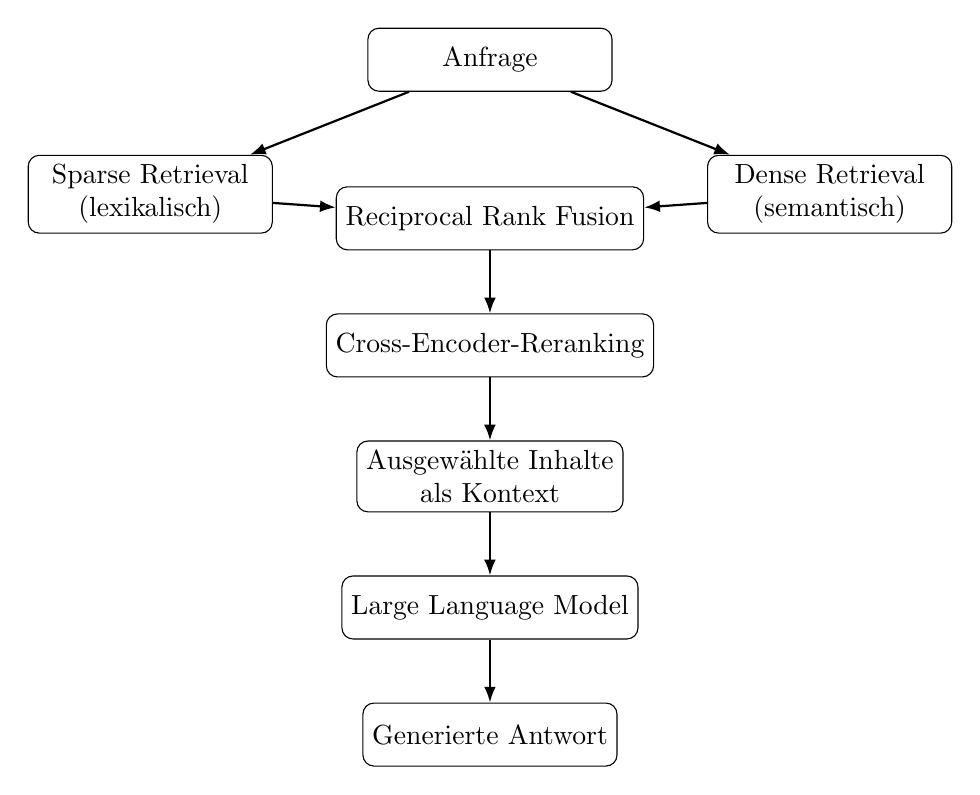
\begin{tikzpicture}[
        node distance=0.8cm and 1.2cm,
        box/.style={
            draw,
            rounded corners,
            align=center,
            minimum width=3.1cm,
            minimum height=0.8cm
        },
        arrow/.style={
            -{Latex[length=2mm]},
            thick
        }
    ]

    \node[box] (query) {Anfrage};

    \node[box, below left=of query] (sparse)
        {Sparse Retrieval\\(lexikalisch)};
    \node[box, below right=of query] (dense)
        {Dense Retrieval\\(semantisch)};

    \node[box, below=1.2cm of query] (rrf)
        {Reciprocal Rank Fusion};

    \node[box, below=of rrf] (rerank)
        {Cross-Encoder-Reranking};

    \node[box, below=of rerank] (context)
        {Ausgewählte Inhalte\\als Kontext};

    \node[box, below=of context] (llm)
        {Large Language Model};

    \node[box, below=of llm] (answer)
        {Generierte Antwort};

    \draw[arrow] (query) -- (sparse);
    \draw[arrow] (query) -- (dense);
    \draw[arrow] (sparse) -- (rrf);
    \draw[arrow] (dense) -- (rrf);
    \draw[arrow] (rrf) -- (rerank);
    \draw[arrow] (rerank) -- (context);
    \draw[arrow] (context) -- (llm);
    \draw[arrow] (llm) -- (answer);

    \end{tikzpicture}
    \caption{Schematischer Ablauf einer hybriden RAG-Pipeline mit Reranking.}
    \label{fig:rag_pipeline_grundlagen}
\end{figure}

\subsection{Evaluation LLM-basierter Dialogsysteme}
\label{subsec:llm_evaluation}

Die Bewertung von LLM-basierten Dialogsystemen unterscheidet sich von Aufgaben, für die eine eindeutig definierte Zielausgabe vorliegt. Insbesondere bei offenen Dialogen können mehrere inhaltlich und sprachlich unterschiedliche Antworten eine gestellte Anforderung erfüllen. Für solche Ausgaben kann ein Large Language Model selbst als Evaluator eingesetzt werden. Dieses Verfahren wird als \textit{LLM-as-a-Judge} bezeichnet.

\subsubsection{LLM-as-a-Judge}
\label{subsubsec:llm_judge}

Beim LLM-as-a-Judge wird ein Large Language Model eingesetzt, um die Ausgabe eines zu untersuchenden LLM-Systems anhand vorgegebener Bewertungskriterien zu beurteilen. Zheng et al. untersuchen diesen Ansatz für die Evaluation von Chat-Assistenten und verwenden leistungsfähige LLMs sowohl zur Bewertung einzelner Antworten als auch zum Vergleich verschiedener Antworten \cite{Zheng2023LLMJudge}. Damit übernimmt das bewertende Modell eine Funktion, die andernfalls beispielsweise durch menschliche Evaluatoren ausgeführt werden müsste.

Der Ansatz ermöglicht insbesondere die Bewertung von Eigenschaften, die sich nicht ausschließlich durch einen Vergleich mit einer festgelegten Referenzantwort bestimmen lassen. Die Bewertung bleibt jedoch vom eingesetzten Judge-Modell und vom Bewertungsverfahren abhängig. Zheng et al. identifizieren unter anderem einen \textit{Position Bias}, bei dem die Position einer Antwort das Urteil beeinflussen kann, einen \textit{Verbosity Bias}, der ausführlichere Antworten begünstigen kann, sowie einen \textit{Self-Enhancement Bias} zugunsten von Antworten verwandter Modelle \cite{Zheng2023LLMJudge}. LLM-as-a-Judge ist daher nicht als objektive Messung zu verstehen, sondern als modellbasierte Evaluationsmethode, deren Ausgestaltung bei der Interpretation der Ergebnisse berücksichtigt werden muss.

\subsubsection{Multi-Turn-Evaluation und ConversationalTestCase}
\label{subsubsec:conversational_testcase}

Bei einem Dialogsystem hängt die Qualität einer Antwort nicht ausschließlich von der unmittelbar vorhergehenden Eingabe ab. Aussagen, Anforderungen oder Informationen aus früheren Gesprächsschritten können für spätere Antworten weiterhin maßgeblich sein. Eine isolierte Bewertung einzelner Input-Output-Paare kann deshalb Eigenschaften wie die Berücksichtigung des Gesprächskontexts oder ein konsistentes Verhalten über den gesamten Dialog nur eingeschränkt erfassen. DeepEval unterscheidet hierzu zwischen Single-Turn- und Multi-Turn-Evaluation und verwendet für letztere den \texttt{ConversationalTestCase} \cite{DeepEvalConversationalTestCase}.

Ein \texttt{ConversationalTestCase} repräsentiert eine vollständige Konversation als Folge von \texttt{Turn}-Objekten. Ein Turn enthält insbesondere die jeweilige Rolle, beispielsweise \texttt{user} oder \texttt{assistant}, sowie den Inhalt der Nachricht. Zusätzlich kann ein Conversational Test Case Angaben zum Szenario, zum erwarteten Ergebnis, zum verfügbaren Kontext oder zur vorgesehenen Rolle des Chatbots enthalten \cite{DeepEvalConversationalTestCase}. Die Konversation bildet damit die gemeinsame Evaluationsgrundlage für Metriken, deren Bewertung sich über mehrere Interaktionen erstreckt.

Diese Betrachtung ist insbesondere für Tutor-Chatbots erforderlich. Ein einzelner Turn kann für sich betrachtet einer vorgesehenen Tutorstrategie entsprechen, während das System diese Strategie in späteren Gesprächsschritten nicht fortführt. Die Multi-Turn-Evaluation ermöglicht deshalb die Untersuchung, ob gewünschte Eigenschaften über den Gesprächsverlauf hinweg erhalten bleiben.

\subsubsection{Conversational G-Eval}
\label{subsubsec:conversational_geval}

Für Anforderungen, für die keine vorgegebene Metrik existiert, stellt DeepEval mit \texttt{ConversationalGEval} eine anpassbare LLM-as-a-Judge-Metrik für Multi-Turn-Konversationen bereit \cite{DeepEvalConversationalGEval}. Hierzu wird ein natürlichsprachliches Bewertungskriterium definiert, anhand dessen ein Judge-Modell die im \texttt{ConversationalTestCase} enthaltene Konversation beurteilt. Im Gegensatz zu einer auf einzelne Antworten beschränkten Bewertung kann damit das Verhalten über den gesamten Gesprächsverlauf Gegenstand des Bewertungskriteriums sein.

Dadurch können anwendungsspezifische Qualitätsanforderungen operationalisiert werden, für die keine allgemeingültige Metrik vorhanden ist. Im Kontext eines Tutors können solche Kriterien beispielsweise das didaktische Verhalten oder die Einhaltung bestimmter Gesprächsstrategien betreffen. Die konkrete Formulierung dieser Kriterien sowie ihre Verwendung für die Evaluation des in dieser Arbeit untersuchten Tutors werden im Methodikkapitel beschrieben.

\subsubsection{Vordefinierte Multi-Turn-Metriken}
\label{subsubsec:multiturn_metrics}

Neben frei definierbaren Kriterien stellt DeepEval vordefinierte Metriken für wiederkehrende Qualitätsdimensionen von Multi-Turn-Systemen bereit. Für die vorliegende Untersuchung sind insbesondere \textit{Role Adherence}, \textit{Turn Contextual Relevancy} und \textit{Turn Faithfulness} relevant.

Die \textit{Role Adherence} bewertet, in welchem Maß ein Dialogsystem die ihm vorgegebene Rolle über den Gesprächsverlauf hinweg einhält. Hierzu werden die Assistant-Turns unter Berücksichtigung der vorausgehenden Konversation mit der im \texttt{ConversationalTestCase} definierten \texttt{chatbot\_role} verglichen \cite{DeepEvalRoleAdherence}. Die Metrik ermöglicht damit eine Bewertung, ob das gewünschte Rollenverhalten auch über mehrere Gesprächsschritte hinweg beibehalten wird.

Für die Bewertung der RAG-Komponente werden \textit{Turn Contextual Relevancy} und \textit{Turn Faithfulness} herangezogen. \textit{Turn Contextual Relevancy} untersucht, ob der für einen Turn abgerufene Retrieval-Kontext für die jeweilige Nutzereingabe relevant ist \cite{DeepEvalTurnContextualRelevancy}. Die Metrik richtet sich damit auf die Qualität der bereitgestellten Kontextinformationen.

\textit{Turn Faithfulness} betrachtet dagegen die Beziehung zwischen dem Retrieval-Kontext und der generierten Antwort. Bewertet wird, ob die Aussagen des Assistenten durch die für den jeweiligen Turn bereitgestellten Informationen gestützt werden \cite{DeepEvalTurnFaithfulness}. Während \textit{Turn Contextual Relevancy} somit die Relevanz des abgerufenen Kontexts bewertet, untersucht \textit{Turn Faithfulness}, ob die Antwort auf diesem Kontext basiert.

Die drei Metriken adressieren damit unterschiedliche Qualitätsdimensionen des Dialogsystems: \textit{Role Adherence} die Einhaltung der vorgesehenen Tutorrolle, \textit{Turn Contextual Relevancy} die Relevanz der abgerufenen Inhalte und \textit{Turn Faithfulness} deren Nutzung bei der Antwortgenerierung. Die konkrete Zuordnung der Metriken zu den Forschungsfragen wird im Methodikkapitel beschrieben.

\section{Untersuchungsgegenstand}
\label{sec:untersuchungsgegenstand}
 
Die Untersuchung betrachtet sowohl das Tutorverhalten als auch die Bereitstellung des fachlichen Kontexts. RQ1 adressiert den Vergleich unterschiedlicher Systemprompt-Varianten hinsichtlich ihres sokratischen Tutorverhaltens, während RQ2 die untersuchten RAG-Konfigurationen gegenüberstellt. Die Grundlage beider Untersuchungen ist die im Folgenden dargestellte RAG-Pipeline.
 
\subsection{Die RAG-Pipeline}
\label{subsec:rag_pipeline}
 
Als Untersuchungsgegenstand dient eine Open-WebUI-kompatible RAG-Pipeline, die OpenAI-kompatible Chat-Completion-Anfragen verarbeitet und Qdrant als Vektordatenbank für das Retrieval verwendet. Die Pipeline unterstützt Dense, Sparse und Hybrid Retrieval sowie Reciprocal Rank Fusion (RRF) und optionales Cross-Encoder-Reranking. Darüber hinaus können Kontextinformationen aus Moodle in die Verarbeitung einbezogen werden.
 
Der grundsätzliche Ablauf ist in Abbildung~\ref{fig:system_pipeline} dargestellt. Nach Eingang einer Nutzeranfrage werden zunächst die Request-Parameter und die aktuelle Frage bestimmt. Abhängig von der gewählten Retrieval-Konfiguration wird die Anfrage anschließend über Dense Retrieval, Sparse Retrieval oder eine Kombination beider Verfahren verarbeitet. Im hybriden Modus werden Dense- und Sparse-Repräsentationen parallel erzeugt. Die resultierenden Rankings werden mittels RRF zusammengeführt. Dabei wird, sofern verfügbar, die serverseitige Fusion durch Qdrant verwendet; andernfalls erfolgt die Fusion lokal innerhalb der Pipeline.
 
Die resultierenden Kandidaten werden zusammengeführt und gegebenenfalls dedupliziert. Optional kann anschließend ein Cross-Encoder die Kandidaten erneut bewerten und neu sortieren. Nach dem Retrieval beziehungsweise Reranking werden ein Score-Threshold sowie ein finales Trefferlimit angewendet. Die verbleibenden Chunks bilden die Grundlage für den RAG-Kontext. Dabei begrenzt ein Kontextbudget die Menge der tatsächlich an das Sprachmodell übergebenen Inhalte, sodass nicht zwingend jeder finale Retrieval-Treffer Bestandteil des LLM-Kontexts ist.
 
\begin{figure}[htbp]
    \centering
    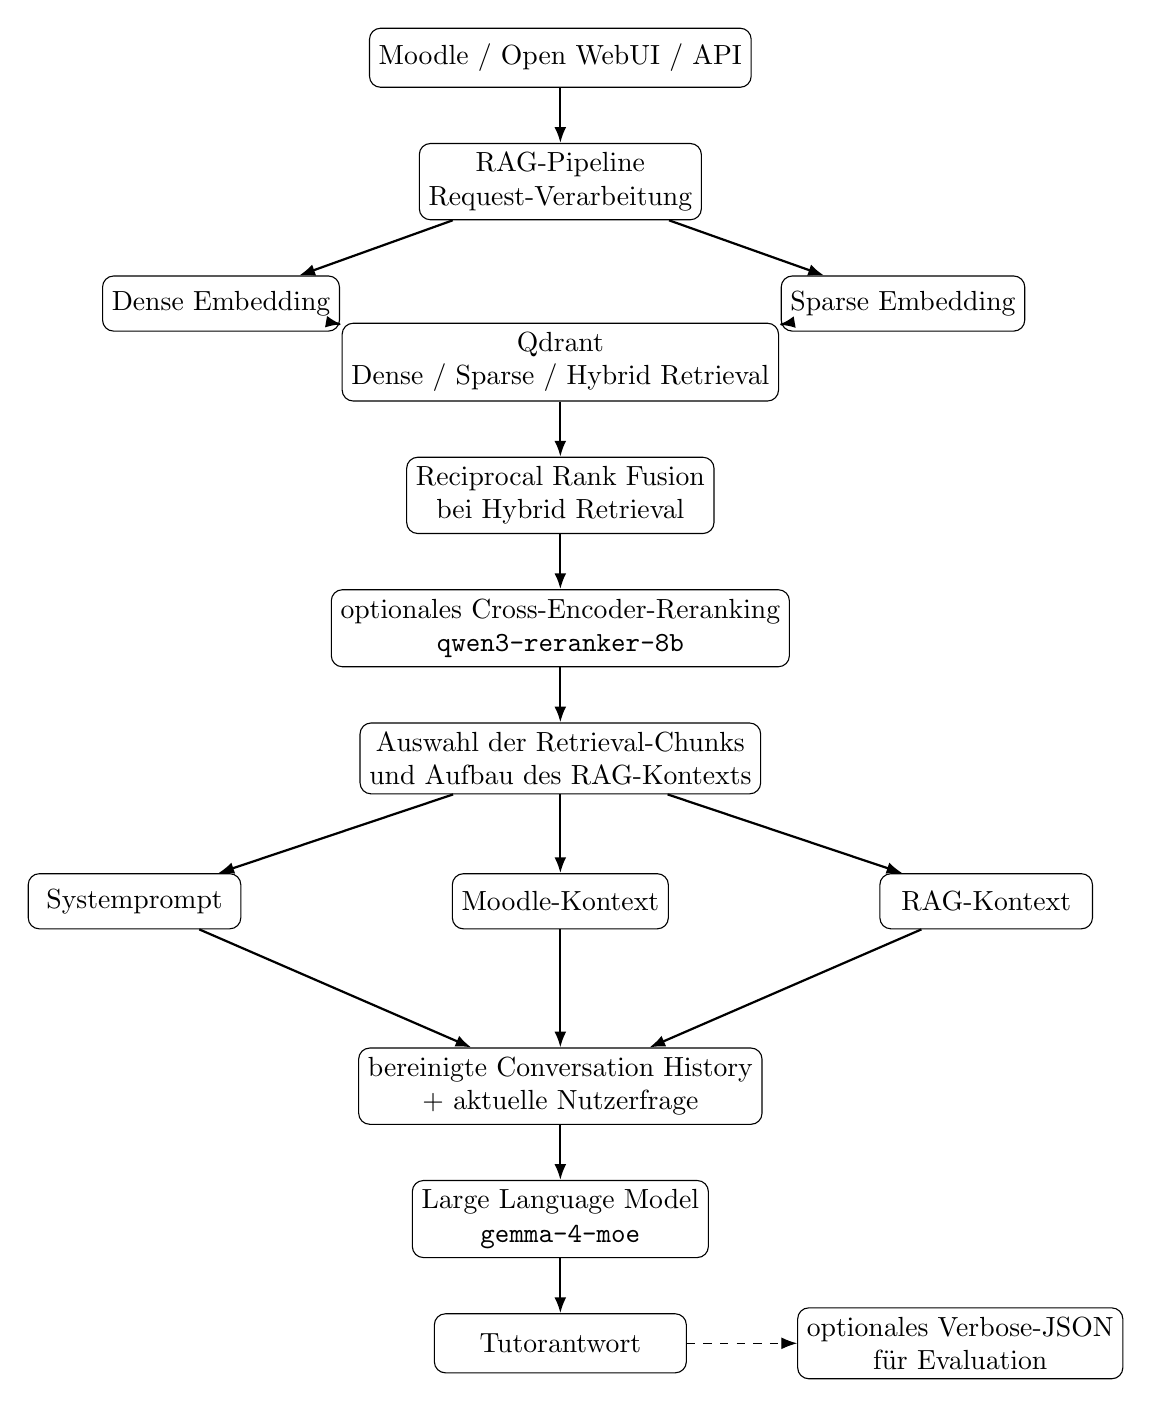
\begin{tikzpicture}[
        node distance=0.7cm and 1.0cm,
        box/.style={
            draw,
            rounded corners,
            align=center,
            minimum width=3.2cm,
            minimum height=0.75cm
        },
        smallbox/.style={
            draw,
            rounded corners,
            align=center,
            minimum width=2.7cm,
            minimum height=0.7cm
        },
        arrow/.style={
            -{Latex[length=2mm]},
            thick
        },
        optional/.style={
            -{Latex[length=2mm]},
            dashed
        }
    ]
 
    % Eingang
    \node[box] (client)
        {Moodle / Open WebUI / API};
 
    \node[box, below=of client] (pipeline)
        {RAG-Pipeline\\Request-Verarbeitung};
 
    % Retrieval
    \node[smallbox, below left=of pipeline] (dense)
        {Dense Embedding};
 
    \node[smallbox, below right=of pipeline] (sparse)
        {Sparse Embedding};
 
    \node[box, below=1.3cm of pipeline] (qdrant)
        {Qdrant\\Dense / Sparse / Hybrid Retrieval};
 
    \node[box, below=of qdrant] (rrf)
        {Reciprocal Rank Fusion\\bei Hybrid Retrieval};
 
    \node[box, below=of rrf] (rerank)
        {optionales Cross-Encoder-Reranking\\
        \texttt{qwen3-reranker-8b}};
 
    \node[box, below=of rerank] (context)
        {Auswahl der Retrieval-Chunks\\und Aufbau des RAG-Kontexts};
 
    % Promptbestandteile
    \node[smallbox, below left=1.0cm and 1.5cm of context] (system)
        {Systemprompt};
 
    \node[smallbox, below=1.0cm of context] (moodle)
        {Moodle-Kontext};
 
    \node[smallbox, below right=1.0cm and 1.5cm of context] (rag)
        {RAG-Kontext};
 
    \node[box, below=1.5cm of moodle] (history)
        {bereinigte Conversation History\\+ aktuelle Nutzerfrage};
 
    \node[box, below=of history] (llm)
        {Large Language Model\\\texttt{gemma-4-moe}};
 
    \node[box, below=of llm] (answer)
        {Tutorantwort};
 
    % Verbose
    \node[smallbox, right=1.4cm of answer] (verbose)
        {optionales Verbose-JSON\\für Evaluation};
 
    % Pfeile
    \draw[arrow] (client) -- (pipeline);
 
    \draw[arrow] (pipeline) -- (dense);
    \draw[arrow] (pipeline) -- (sparse);
 
    \draw[arrow] (dense) -- (qdrant);
    \draw[arrow] (sparse) -- (qdrant);
 
    \draw[arrow] (qdrant) -- (rrf);
    \draw[arrow] (rrf) -- (rerank);
    \draw[arrow] (rerank) -- (context);
 
    \draw[arrow] (context) -- (system);
    \draw[arrow] (context) -- (moodle);
    \draw[arrow] (context) -- (rag);
 
    \draw[arrow] (system) -- (history);
    \draw[arrow] (moodle) -- (history);
    \draw[arrow] (rag) -- (history);
 
    \draw[arrow] (history) -- (llm);
    \draw[arrow] (llm) -- (answer);
 
    \draw[optional] (answer) -- (verbose);
 
    \end{tikzpicture}
 
    \caption{Architektur und Verarbeitungsschritte der untersuchten RAG-Pipeline in Version 1.7.0.}
    \label{fig:system_pipeline}
\end{figure}
 
Für die Generierung wird der Prompt aus mehreren Bestandteilen zusammengesetzt. Im RAG-Pfad werden zunächst der aktive Systemprompt, anschließend ein optionaler Moodle-Kontext und der aus dem Retrieval erzeugte RAG-Kontext eingefügt. Darauf folgen die bereinigte bisherige Gesprächshistorie und die aktuelle Nutzerfrage. Die Pipeline ermöglicht damit, sowohl retrieved Informationen als auch den bisherigen Gesprächsverlauf bei der Generierung einer Tutorantwort zu berücksichtigen.
 
Version 1.7.0 stellt zusätzlich einen Verbose-Modus für Non-Streaming-Anfragen bereit. Dieser gibt unter anderem Informationen über die Vektorisierung, die Retrieval- und Fusionsergebnisse, das Reranking, die tatsächlich an das LLM übergebenen Nachrichten sowie die rohe und finale Modellantwort strukturiert aus. Der Verbose-Modus greift dabei auf bereits während der regulären Verarbeitung erzeugte Daten zurück und führt keine zusätzlichen Retrieval-, Embedding-, Reranking- oder LLM-Aufrufe aus. Dadurch können die einzelnen Verarbeitungsschritte für die spätere Evaluation nachvollzogen werden. Die für die Untersuchung variierten Retrieval- und Reranking-Konfigurationen werden in Abschnitt~\ref{subsec:rag_konfigurationen} beschrieben.
 
 
\subsection{Die Prompt-Varianten für RQ1}
\label{subsec:prompt_varianten}
 
Zur Beantwortung von RQ1 werden vier Varianten des Systemprompts miteinander verglichen. Sie unterscheiden sich hinsichtlich des Umfangs der Instruktionen, der Strukturierung des sokratischen Dialogs und der Anpassung an den konkreten Einsatz im Elektrotechniklabor. Dadurch soll untersucht werden, welchen Einfluss die Ausgestaltung des Systemprompts auf das resultierende Tutorverhalten hat. Die vollständigen Wortlaute der verwendeten Prompts sind in Anhang~\ref{app:prompts} dokumentiert.
 
Die \textit{Baseline ohne Systemprompt} enthält keine zusätzliche Instruktion zur Rolle oder zum Verhalten des Modells. Sie dient als Referenz, um zu untersuchen, welches Tutorverhalten das Sprachmodell ohne explizite Vorgaben zum sokratischen Vorgehen zeigt.
 
Der \textit{Minimale sokratische Prompt} definiert das Modell als sokratischen Tutor für Elektrotechnik. Vorgegeben wird lediglich, Gegenfragen anstelle direkter Antworten zu stellen und Studierende durch Fragen zur eigenständigen Erkenntnis zu führen. Weitere Regeln zum Ablauf des Gesprächs oder zum Umgang mit bestimmten Situationen werden nicht festgelegt.
 
Der \textit{Strukturierte sokratische Prompt} konkretisiert den Ablauf des sokratischen Dialogs. Ausgangspunkt soll eine konkrete Erfahrung der studierenden Person sein, aus der schrittweise Begriffe, Urteile sowie zugrunde liegende Überzeugungen und Prinzipien herausgearbeitet werden. Der Tutor soll sich dabei weitgehend aus der direkten fachlichen Problemlösung heraushalten, Gegenperspektiven einbringen und die studierende Person durch Fragen zum eigenständigen Weiterdenken anregen. Zusätzlich enthält der Prompt die Vorgabe, die Lösung einer Quizfrage nicht direkt oder indirekt preiszugeben.
 
Der \textit{Domänenspezifische In-Lab-Tutorprompt} überträgt das sokratische Tutorverhalten auf Situationen während eines Elektrotechniklabors. Neben der Förderung eigenständigen Denkens enthält er Vorgaben zur Berücksichtigung des Vorwissens, zur Entwicklung und Prüfung eigener Fehlerhypothesen sowie zur Begrenzung der Informationsmenge und der Anzahl der Impulse pro Antwort. Darüber hinaus definiert der Prompt Eskalationsregeln für sicherheitsrelevante oder durch die Laborbetreuung zu klärende Situationen.
 
Tabelle~\ref{tab:prompt_varianten} fasst die wesentlichen Unterschiede der vier Varianten zusammen.
 
\begin{table}[htbp]
    \centering
    \caption{Für RQ1 untersuchte Prompt-Varianten.}
    \label{tab:prompt_varianten}
 
    \renewcommand{\arraystretch}{1.25}
 
    \begin{tabularx}{\linewidth}{
        @{}
>{\centering\arraybackslash}p{0.8cm}
>{\raggedright\arraybackslash}p{3.7cm}
>{\centering\arraybackslash}p{1.8cm}
>{\raggedright\arraybackslash}X
        @{}
    }
        \toprule
        \textbf{ID} &
        \textbf{Variante} &
        \textbf{Umfang} &
        \textbf{Schwerpunkt} \\
        \midrule
 
        A &
        Baseline ohne Systemprompt &
        keiner &
        Keine explizite Vorgabe eines sokratischen Tutorverhaltens. \\[0.3em]
 
        B &
        Minimaler sokratischer Prompt &
        gering &
        Definition der Tutorrolle sowie Vorgabe von Gegenfragen und Förderung eigenständiger Erkenntnis. \\[0.3em]
 
        C &
        Strukturierter sokratischer Prompt &
        hoch &
        Vorgegebener sokratischer Gesprächsablauf und Vermeidung direkter Lösungsweitergabe. \\[0.3em]
 
        D &
        Domänenspezifischer In-Lab-Tutorprompt &
        hoch &
        Anpassung des Tutorverhaltens an das Elektrotechniklabor mit Hypothesenbildung, begrenzten Impulsen und Eskalationsregeln. \\
 
        \bottomrule
    \end{tabularx}
\end{table}
 
Die vier Varianten bilden damit unterschiedliche Grade der Steuerung durch den Systemprompt ab. Während die Baseline vollständig auf eine sokratische Instruktion verzichtet und der minimale Prompt lediglich das Grundprinzip vorgibt, operationalisieren die beiden umfangreicheren Varianten das gewünschte Tutorverhalten stärker. Der strukturierte sokratische Prompt fokussiert dabei den Ablauf des sokratischen Dialogs, während der domänenspezifische In-Lab-Tutorprompt zusätzlich Anforderungen des konkreten Laborkontexts berücksichtigt. Die methodische Durchführung des Vergleichs wird in Kapitel~\ref{sec:methodik} beschrieben.
 
\subsection{RAG-Konfigurationen für RQ2}
\label{subsec:Die RAG-Konfigurationen}
 
Zur Beantwortung von RQ2 werden unterschiedliche Konfigurationen der in Abschnitt~\ref{subsec:rag_pipeline} beschriebenen RAG-Pipeline untersucht. Die Varianten unterscheiden sich hinsichtlich der verwendeten Wissensbasis, des Retrieval-Verfahrens und des Einsatzes eines Cross-Encoder-Rerankings. Dadurch kann untersucht werden, welchen Einfluss diese Komponenten auf die Qualität des bereitgestellten Retrieval-Kontexts und der darauf basierenden Antworten haben.
 
Als Wissensbasis werden eine Collection mit Vorlesungsinhalten, eine Collection mit Laborinhalten sowie die Kombination beider Collections betrachtet. Für das Retrieval kommen Dense, Sparse und Hybrid Retrieval zum Einsatz. Beim hybriden Verfahren werden Dense und Sparse Retrieval kombiniert und die resultierenden Ranglisten mittels Reciprocal Rank Fusion zusammengeführt. In ausgewählten Konfigurationen wird anschließend zusätzlich das in Abschnitt~\ref{subsec:rag_pipeline} beschriebene Cross-Encoder-Reranking angewendet.
 
Neben den RAG-Konfigurationen wird eine \textit{LLM-only}-Variante untersucht. Bei dieser wird keine Collection ausgewählt, sodass Retrieval und Reranking vollständig übersprungen werden. Sie dient als Referenz für die Antwortgenerierung ohne zusätzlich bereitgestellten Retrieval-Kontext.
 
Tabelle~\ref{tab:rag_konfigurationen} zeigt die für RQ2 untersuchten Konfigurationen.
 
\begin{table}[htbp]
    \centering
    \caption{Für RQ2 untersuchte RAG-Konfigurationen.}
    \label{tab:rag_konfigurationen}
    \renewcommand{\arraystretch}{1.2}
    \begin{tabularx}{\linewidth}{
        @{}
        >{\raggedright\arraybackslash}X
        >{\raggedright\arraybackslash}p{3.0cm}
        >{\raggedright\arraybackslash}p{2.6cm}
        >{\centering\arraybackslash}p{1.8cm}
        @{}
    }
        \toprule
        \textbf{Variante} &
        \textbf{Wissensbasis} &
        \textbf{Retrieval} &
        \textbf{Reranking} \\
        \midrule
 
        Beide -- Hybrid &
        Vorlesung + Labor &
        Hybrid &
        Nein \\
 
        Beide -- Sparse &
        Vorlesung + Labor &
        Sparse &
        Nein \\
 
        Beide -- Hybrid + Reranking &
        Vorlesung + Labor &
        Hybrid &
        Ja \\
 
        Vorlesung -- Hybrid + Reranking &
        Vorlesung &
        Hybrid &
        Ja \\
 
        Labor -- Hybrid + Reranking &
        Labor &
        Hybrid &
        Ja \\
 
        Beide -- Dense &
        Vorlesung + Labor &
        Dense &
        Nein \\
 
        Labor -- Dense &
        Labor &
        Dense &
        Nein \\
 
        Vorlesung -- Dense &
        Vorlesung &
        Dense &
        Nein \\
 
        LLM-only &
        keine &
        kein Retrieval &
        Nein \\
 
        \bottomrule
    \end{tabularx}
\end{table}
 
Die Auswahl der Varianten ermöglicht mehrere Vergleichsperspektiven. Durch die Dense-, Sparse- und Hybrid-Konfigurationen werden unterschiedliche Retrieval-Ansätze gegenübergestellt. Die Varianten mit beiden Collections und mit getrennten Vorlesungs- beziehungsweise Laborinhalten erlauben zusätzlich eine Untersuchung des Einflusses der zugrunde liegenden Wissensbasis. Der Vergleich der hybriden Varianten mit und ohne Reranking dient schließlich dazu, den zusätzlichen Einfluss des Cross-Encoder-Rerankings zu betrachten. Die konkrete Durchführung der Evaluation und die hierfür verwendeten Metriken werden in Kapitel~\ref{sec:methodik} beschrieben. Aufgrund des hohen Tokenaufwands und der damit verbundenen Kosten des OpenAI-Zugangs konnte die Evaluation nicht für alle neun vorgesehenen RAG-Konfigurationen vollständig durchgeführt werden. Versuche, die verbleibenden Konfigurationen über die lokale Infrastruktur der Hochschule zu evaluieren, erwiesen sich aufgrund sehr langer Laufzeiten und erreichter Systemgrenzen ebenfalls als nicht praktikabel, sodass nur die Varianten beide\_sparse, beide\_dense, labor\_dense, vorlesung\_dense und llm\_only ausgewertet wurden.
\section{Methodik}
\label{sec:methodik}

Gegenstand der vorliegenden Untersuchung ist die Evaluation eines sokratischen
KI\-Tutors, der auf einer Retrieval\-Augmented\-Generation\-Pipeline (RAG) aufsetzt.
Ziel ist es, das Zusammenspiel von Prompting und Retrieval\-Konfiguration systematisch
zu bewerten. Die Untersuchung folgt einem explorativen, experimentellen
Evaluationsdesign, das zwei Forschungsfragen getrennt adressiert: den Einfluss
verschiedener sokratischer Prompts (RQ1) sowie den Einfluss verschiedener
RAG\-Konfigurationen (RQ2). Beide Fragen werden über dieselbe technische
Evaluationsarchitektur beantwortet, jedoch in zwei voneinander unabhängigen
Auswertungslinien, sodass jeweils nur ein Faktor variiert wird.

\subsection{Untersuchungsdesign}
\label{subsec:design}

Die Evaluation ist als automatisierte, mehrstufige Dialogbewertung angelegt. Für jedes
Testszenario wird ein Multi\-Turn\-Gespräch zwischen einer simulierten studierenden
Person und dem RAG\-gestützten Tutor erzeugt und anschließend anhand eines definierten
Metrik\-Sets bewertet. Die Wahl eines simulationsbasierten Multi\-Turn\-Designs ergibt
sich unmittelbar aus dem Untersuchungsgegenstand: Da sokratisches Tutoring ein
dialogisches, über mehrere Gesprächsrunden verlaufendes Vorgehen ist, lässt es sich
nicht anhand einzelner Frage\-Antwort\-Paare, sondern nur im Verlauf eines Gesprächs
angemessen beurteilen \cite{QUELLE_SOKRATIK}.

Zur klaren Trennung der Forschungsfragen wurden zwei separate Evaluationslinien
umgesetzt. In der ersten Linie (RQ1) wird bei konstant gehaltener RAG\-Konfiguration
der System\-Prompt variiert. Bewertet wird die \emph{\texttt{no\_Prompt}
\texttt{stock\_prompt}tät} des
Gesprächsverlaufs. In der zweiten Linie (RQ2) wird bei konstant gehaltenem Prompt die
RAG\-Konfiguration variiert und die \emph{Retrieval\-Qualität} bewertet. Durch die
Beschränkung auf jeweils einen variierten Faktor je Linie können die beobachteten
Effekte den Prompts bzw. den Konfigurationen zugeordnet werden.

\subsection{Untersuchungsgegenstand und Datengrundlage}
\label{subsec:gegenstand}

Das zu evaluierende System (System under Test) ist eine OpenWebUI\-kompatible
RAG\-Pipeline, die einen Qdrant\-Vektorspeicher, ein Cross\-Encoder\-Reranking sowie
Moodle\-Metadaten anbindet. Als generierendes Sprachmodell nutzt die Pipeline intern
das Modell \texttt{gemma\-4\-26B}. Der fachliche Wissenskorpus liegt in zwei
Qdrant\-Collections vor, die Vorlesungs\- bzw. Labormaterial des Fachgebiets
Elektronik der Hochschule enthalten.

Die Datengrundlage der Evaluation bilden nicht vorab gesammelte Dialoge, sondern
synthetisch erzeugte Gespräche. Grundlage jedes Gesprächs ist ein Testszenario,
das sich aus der Kombination von Themengebiet, Kompetenzniveau der studierenden Person
(Anfänger bzw. Fortgeschritten) und einem charakteristischen Studierenden\-Verhalten
(etwa kooperativ, die Lösung einfordernd oder inhaltlich selbstsicher\-fehlerhaft)
zusammensetzt. Insgesamt ergeben sich daraus 24 Szenarien je Auswertungslinie. Jedes Szenario wird als \emph{Golden} modelliert, das die
Ausgangssituation, eine Beschreibung der zu simulierenden Persona sowie eine feste
Initialfrage enthält. Die Initialfrage wird bewusst wortgleich vorgegeben und nicht
generiert, um über alle Prompts und Konfigurationen hinweg denselben Gesprächseinstieg
und damit die Vergleichbarkeit der Läufe sicherzustellen; die daran anschließenden
Folgefragen werden hingegen dynamisch simuliert.

% =========================================================
% TABELLE 1 · Szenario-Dimensionen
% =========================================================
\begin{table}[htbp]
  \centering
  \caption{Dimensionen der Testszenarien. Die Kombination aus Themengebiet,
  Kompetenzniveau und Studierenden-Verhalten ergibt die simulierten Gespr\"ache.}
  \label{tab:szenario-dimensionen}
  \begin{tabular}{ll}
    \toprule
    \textbf{Dimension} & \textbf{Auspr\"agungen} \\
    \midrule
    Themengebiet & Sperrspannung/Durchbruch der Z-Diode; \\
                 & Spannungsstabilisierung mit Z-Diode; \\
                 & Ohmsches Gesetz und Maschenregel \\
    \addlinespace
    Kompetenzniveau & Anf\"anger, Fortgeschritten \\
    \addlinespace
    Studierenden-Verhalten & kooperativ; gibt schnell auf; \\
                           & fordert die L\"osung ein; \\
                           & \"au{\ss}ert eine Vermutung; \\
                           & selbstsicher, aber inhaltlich falsch \\
    \bottomrule
  \end{tabular}
\end{table}
 
\subsection{Evaluationsarchitektur}
\label{subsec:architektur}

Da der Untersuchungsgegenstand ein Dialog ist, sind neben dem zu bewertenden System zwei
weitere Rollen erforderlich. Die Architektur umfasst somit drei klar getrennte Modelle.
Der Tutor ist die RAG\-Pipeline {gemma\-4\-26B} und beantwortet jeden
Gesprächszug. Der Studenten\-Simulator übernimmt die Rolle der studierenden
Person und erzeugt auf Basis von Szenario, Persona und der jeweils vorangegangenen
Tutor\-Antwort die Folgefragen. Ohne diese Rolle entstünde kein Dialog, sondern
lediglich ein einzelnes Frage\-Antwort\-Paar. Als Simulator wird das Modell
\texttt{gpt\-4o\-mini} eingesetzt, das auf dem verwendeten Endpunkt einen Alias für
\texttt{gemma\-4\-26B} darstellt und somit auf demselben Basismodell wie die
RAG\-Pipeline beruht. Der Judge bewertet den fertigen Dialog. Hierfür wird mit
gpt\-4.1 bewusst ein vom System under Test verschiedenes Modell gewählt, um
einen Selbstbewertungs\-Bias zu vermeiden, bei dem ein Modell anteilig seine eigenen
Ausgaben bewertet \cite{QUELLE_LLM_JUDGE}. Simulator und Judge laufen auf getrennten Endpunkten.
% =========================================================
% ABBILDUNG · Ablauf der Dialog-Simulation
% =========================================================
\begin{figure}[htbp]
  \centering
  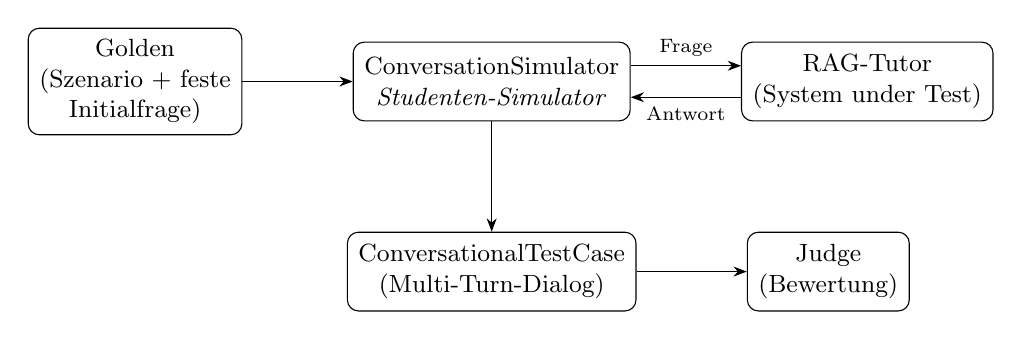
\begin{tikzpicture}[
    node distance=10mm and 14mm,
    box/.style={draw, rounded corners, align=center, minimum height=10mm,
                inner sep=4pt, font=\small},
    lbl/.style={font=\scriptsize},
    >={Stealth[]}
  ]
    \node[box] (golden) {Golden\\(Szenario + feste\\Initialfrage)};
    \node[box, right=of golden] (sim) {ConversationSimulator\\\emph{Studenten-Simulator}};
    \node[box, right=of sim] (rag) {RAG-Tutor\\(System under Test)};
    \node[box, below=14mm of sim] (tc) {ConversationalTestCase\\(Multi-Turn-Dialog)};
    \node[box, right=of tc] (judge) {Judge\\(Bewertung)};
 
    \draw[->] (golden) -- (sim);
    \draw[->] ([yshift=2mm]sim.east) -- node[lbl, above]{Frage} ([yshift=2mm]rag.west);
    \draw[->] ([yshift=-2mm]rag.west) -- node[lbl, below]{Antwort} ([yshift=-2mm]sim.east);
    \draw[->] (sim) -- (tc);
    \draw[->] (tc) -- (judge);
  \end{tikzpicture}
  \caption{Ablauf der Dialog-Simulation: Aus einem Golden erzeugt der
  ConversationSimulator (in der Rolle der studierenden Person) fortlaufend
  Fragen an den RAG-Tutor; der resultierende Multi-Turn-Dialog wird anschlie{\ss}end
  vom Judge bewertet.}
  \label{fig:simulationsablauf}
\end{figure}
\subsection{Verwendete Methoden und Werkzeuge}
\label{subsec:methoden}

Die technische Umsetzung erfolgt in Python unter Verwendung des
Evaluations\-Frameworks DeepEval. Die Multi\-Turn\-Gespräche
werden mit dem ConversationSimulator des Frameworks erzeugt. Ausgehend von der
festen Initialfrage generiert der Simulator über eine festgelegte Anzahl von Runden
fortlaufend Studierenden\-Nachrichten, die über eine Callback\-Schnittstelle an die
RAG\-Pipeline gesendet werden. Die Antwort bildet jeweils den nächsten
Assistant\-Turn. Die Zuordnung von Antworten zu Metriken erfolgt anschließend über
ConversationalTestCase\-Objekte des Frameworks.

Für die kontextbezogenen Metriken wird der tatsächlich abgerufene Retrieval\-Kontext
benötigt. Dieser wird über den Verbose\-Modus der RAG\-Pipeline gewonnen, der bei
deaktiviertem Streaming eine strukturierte Antwort liefert, aus der die finalen
Retrieval\-Chunks samt Text extrahiert und den jeweiligen Antworten zugeordnet werden.
Zwei Aufbereitungsschritte werden dabei transparent gemacht: Zum einen wird der
Kontext für die Bewertung auf eine handhabbare Länge begrenzt, um ein Überschreiten des
Kontextfensters des Judge zu vermeiden; zum anderen wird die mathematische Notation
(LaTeX) für die Bewertung normalisiert, da sie andernfalls die strukturierte Ausgabe
des Judge stört. Beide Eingriffe betreffen ausschließlich die dem Judge übergebene
Kopie; die gespeicherten Gespräche bleiben unverändert.

\subsection{Bewertungskriterien}
\label{subsec:kriterien}

Die Bewertung ist entlang der beiden Forschungsfragen unterschiedlich ausgestaltet.

\subsubsection{Sokratische Qualität (RQ1)}

Sokratisches Tutoring ist ein didaktik\-spezifisches Konstrukt, für das im verwendeten
Framework keine vorgefertigten Metriken existieren. Es wird daher über eigene, mittels
G\-Eval operationalisierte Kriterien bewertet, die jeweils über
explizite Bewertungsschritte und eine dreistufige Bewertungsskala (Rubric) verankert
sind. Verwendet werden die Kriterien \emph{Lösung nicht verraten}, \emph{Sokratische
Rückfragen}, \emph{Schrittweise Lernprogression}, \emph{Niveau\-Anpassung},
\emph{Fachliche Korrektheit}, \emph{Verständnisförderung/Transfer} sowie
\emph{Respektvolle Kommunikation}. Ergänzend wird die im Framework enthaltene Metrik
zur Rollentreue (\emph{RoleAdherence}) als Gegenprüfung herangezogen, da sie die Treue
zur im Testfall hinterlegten sokratischen Rollendefinition misst und damit als einzige
native Metrik das Konstrukt indirekt berührt.

Bewusst nicht verwendet werden Metriken, die dem sokratischen Ziel widersprechen oder es
verfehlen. Dies betrifft insbesondere eine Metrik zur direkten Zielerreichung, die die
unmittelbare Beantwortung der Fachfrage bewertet und damit dem Prinzip, die Lösung
gerade nicht vorwegzunehmen, entgegensteht, sowie eine generische Turn\-Relevanz\-Metrik,
die legitimes sokratisches Umlenken als weniger relevant einstufen kann.

Zur Beantwortung von RQ1 werden vier Prompt-Varianten verglichen, die sich im Grad der didaktischen Steuerung unterscheiden. Der ausführliche sokratische System-Prompt (\texttt{system\_prompt}) spezifiziert die Gesprächsregeln explizit nach dem Framework der Universität. Der minimalistisch-sokratische Prompt (\texttt{minimaler\_sokrat}) enthält nur die Kernanweisung, ohne die Regeln auszuformulieren. Eine Variante ohne steuernden Prompt (\texttt{no\_Prompt}) dient als Referenz ohne sokratische Vorgabe. Die Standard-Variante (\texttt{stock\_prompt}) verwendet einen generischen Tutor-Prompt ohne sokratische Ausrichtung. Die Varianten spannen damit ein Kontinuum von detaillierter über minimale bis hin zu keiner sokratischen Instruktion auf, wodurch sich der Einfluss des Promptings auf die sokratische Qualität untersuchen lässt. Der vollständige Wortlaut der Prompts ist im Anhang dokumentiert.


% =========================================================
% TABELLE 1 · Uebersicht der RQ1-Bewertungskriterien + Fundierung
% =========================================================
\begin{table}[htbp]
    \centering
    \caption{Bewertungskriterien der sokratischen Qualität (RQ1) mit ihrer
    literaturgestützten Fundierung. Sechs Kriterien werden als eigene
    ConversationalGEval-Metriken operationalisiert; die Rollentreue (RoleAdherence)
    wird als native Metrik ergänzend als Gegenprüfung herangezogen.}
    \label{tab:rq1-kriterien}
    \small

    \begin{tabular}{p{3.6cm}p{6.4cm}p{3.4cm}}
        \toprule
        \textbf{Kriterium} &
        \textbf{Gemessenes Konstrukt} \\
        \midrule

        Lösung nicht verraten &
        Führt zur eigenen Erkenntnis, statt die Lösung zu nennen; lässt eigene Denkarbeit. \\

        \addlinespace

        Sokratische Rückfragen &
        Zielgerichtete, offene Fragen -- keine Fragen ,,um der Frage willen``.\\

        \addlinespace

        Schrittweise Lernprogression &
        Neues Wissen in kleinen Schritten auf Vorwissen aufbauend. \\

        \addlinespace

        Niveau-Anpassung &
        Diagnostiziert das Niveau und unterrichtet daran angepasst. \\

        \addlinespace

        Fachliche Korrektheit &
        Real korrekte Fachinhalte; keine erfundenen Formeln/Werte.\\

        \addlinespace

        Verständnisförderung / Transfer &
        Betont wichtige Lernpunkte; fördert Verständnis statt Reproduktion.\\

        \addlinespace

        Respektvolle Kommunikation &
        Ziel ist Lehren, nicht Bloßstellen; keine Beschämung. \\

        \midrule

        RoleAdherence (nativ) &
        Gegenprüfung der Treue zur sokratischen Rollendefinition.\\

        \bottomrule
    \end{tabular}
\end{table}

\subsubsection{Retrieval\-Qualität (RQ2)}

Für den Vergleich der RAG\-Konfigurationen werden die nativen Metriken
\emph{TurnContextualRelevancy} (Passung des abgerufenen Kontexts zur Frage) und
\emph{TurnFaithfulness} (Deckung der Antwort durch den abgerufenen Kontext) verwendet.
Beide beziehen den zuvor extrahierten Retrieval\-Kontext ein und eignen sich damit zur
Unterscheidung von Retrieval\-Konfigurationen.
% Benötigte Pakete (Praeambel):
% \usepackage{booktabs}
% \usepackage{array}

% =========================================================
% TABELLE 1 · RQ2-Bewertungskriterien (Retrieval-Qualitaet)
% =========================================================
\begin{table}[htbp]
  \centering
  \caption{Bewertungskriterien der Retrieval-Qualit\"at (RQ2). Die beiden Metriken sind
  native DeepEval-Metriken und beziehen den tats\"achlich abgerufenen
  \texttt{retrieval\_context} ein; die Abdeckung und die effektive Retrieval-G\"ute
  werden daraus abgeleitet.}
  \label{tab:rq2-kriterien}
  \small
  \begin{tabular}{p{4.0cm}p{2.0cm}p{7.0cm}}
    \toprule
    \textbf{Kennzahl} & \textbf{Herkunft} & \textbf{Gemessenes Konstrukt} \\
    \midrule
    TurnContextualRelevancy & nativ & Passung des abgerufenen Kontexts zur jeweiligen Frage. \\
    \addlinespace
    TurnFaithfulness        & nativ & Deckung der Antwort durch den abgerufenen Kontext (Grounding). \\
    \addlinespace
    Retrieval-Abdeckung     & abgeleitet & Anteil der Antworten mit tats\"achlich abgerufenem Kontext (aus den Konversationsdaten). \\
    \addlinespace
    Effektive Retrieval-G\"ute & abgeleitet & Produkt aus Abdeckung und Kontext-Relevanz; ber\"ucksichtigt, wie oft \emph{und} wie gut Kontext abgerufen wird. \\
    \bottomrule
  \end{tabular}
\end{table}

% =========================================================
% TABELLE 2 · Untersuchte RAG-Konfigurationen (Testmatrix RQ2)
% =========================================================
\begin{table}[htbp]
  \centering
  \caption{Untersuchte RAG-Konfigurationen (RQ2). Variiert werden die einbezogenen
  Collections, der Retrieval-Modus und der Einsatz des Cross-Encoder-Rerankings; eine
  reine LLM-Konfiguration ohne Retrieval dient als Referenz.}
  \label{tab:rq2-konfigurationen}
  \small
  \begin{tabular}{lp{4.2cm}p{2.6cm}c}
    \toprule
    \textbf{Konfiguration} & \textbf{Collections} & \textbf{Retrieval} & \textbf{Rerank} \\
    \midrule
    llm\_only                 & --                       & --            & Nein \\
    labor\_dense              & Labor                    & dense         & Nein \\
    vorlesung\_dense          & Vorlesung                & dense         & Nein \\
    beide\_dense              & Labor, Vorlesung         & dense         & Nein \\
    beide\_sparse             & Labor, Vorlesung         & sparse        & Nein \\
    beide\_hybrid             & Labor, Vorlesung         & dense, sparse & Nein \\
    beide\_hybrid\_rerank     & Labor, Vorlesung         & dense, sparse & Ja \\
    labor\_hybrid\_rerank     & Labor                    & dense, sparse & Ja \\
    vorlesung\_hybrid\_rerank & Vorlesung                & dense, sparse & Ja \\
    \bottomrule
  \end{tabular}
\end{table}
\subsubsection{Aggregation und Gate\-Logik}

Zur Beantwortung von RQ1 wird aus den G\-Eval\-Kriterien je Gespräch ein gewichteter
Gesamtscore gebildet [PLATZHALTER: konkrete Gewichte angeben und begründen]. Da eine
Lösungspreisgabe für einen sokratischen Tutor kein untergeordneter Mangel, sondern eine
Verletzung der Kernanforderung darstellt, werden die Kriterien \emph{Lösung nicht
verraten} und \emph{Fachliche Korrektheit} zusätzlich als primäre, nicht durch andere
Kriterien kompensierbare Anforderungen behandelt. Statt eines einfachen Mittelwerts,
der eine solche Verletzung durch gute Werte in anderen Kriterien kaschieren würde, wird
daher die Einhaltungsrate dieser Kernanforderungen als eigenständige Kennzahl berichtet.
Für RQ2 werden die Konfigurationen anhand der Mittelwerte der Retrieval\-Metriken sowie
der Retrieval\-Abdeckung, also des Anteils der Antworten mit tatsächlich abgerufenem
Kontext, verglichen.

\subsection{Durchführung}
\label{subsec:durchfuehrung}

Die Durchführung erfolgt zweiphasig und je Prompt\-Version bzw. Konfiguration getrennt:
Zunächst werden alle Gespräche simuliert, anschließend werden sie bewertet. Diese
Trennung erlaubt es, die netz\- und laufzeitintensive Simulation gegen den
RAG\-Endpunkt einmalig durchzuführen und die Judge\-Bewertung unabhängig davon zu
wiederholen. Zur Sicherstellung der Reproduzierbarkeit werden die simulierten Gespräche
je Konversation atomar zwischengespeichert; über eine deterministische Konversations\-ID
wird ein unterbrochener Lauf beim Neustart fortgesetzt, ohne bereits erzeugte Gespräche
neu zu berechnen. Die Bewertungsergebnisse werden fortlaufend je Metrik protokolliert
und ebenfalls fortsetzbar geschrieben.

Für RQ1 werden [PLATZHALTER: Anzahl] Prompt\-Varianten bei einer festen
RAG\-Konfiguration ausgewertet. Für RQ2 wird ein fester sokratischer Prompt mit einer
Matrix aus neun RAG\-Konfigurationen kombiniert, die sich in den einbezogenen
Collections, im Retrieval\-Modus (dense, sparse, hybrid) und im Einsatz des
Cross\-Encoder\-Rerankings unterscheiden und zusätzlich eine reine LLM\-Konfiguration
ohne Retrieval als Referenz umfassen. Zur Steuerung der Endpunkt\-Auslastung wird ein
gemeinsamer Rate\-Limiter eingesetzt; transiente Fehler (etwa Rate\-Limits oder
Timeouts) werden mit ansteigender Wartezeit wiederholt, deterministische Fehler
hingegen unmittelbar protokolliert.

Die Auswertung erfolgt anschließend automatisiert: Aus den protokollierten Rohdaten
werden je Auswertungslinie die beschriebenen Kennzahlen berechnet und zur weiteren
Analyse [PLATZHALTER: verwendete Auswertungs\-/Visualisierungswerkzeuge, z.\,B. pandas]
aufbereitet.

\subsection{Gütekriterien und methodische Einschränkungen}
\label{subsec:limitationen}

Sämtliche Bewertungen sind Urteile eines LLM\-Judge und damit modellabhängig; Ergebnisse
verschiedener Judge\-Modelle sind nicht unmittelbar vergleichbar. Die selbst definierten
G\-Eval\-Kriterien sind projektspezifisch und wurden [PLATZHALTER: Angabe, ob und wie
eine Validierung, z.\,B. eine manuelle Nachbewertung einer Stichprobe, durchgeführt
wurde] abgesichert. Simulator und RAG\-Tutor beruhen auf demselben Basismodell, was
durch die auf dem verwendeten Endpunkt verfügbaren Modelle bedingt ist; die methodisch
zentrale Trennung zwischen Judge und System under Test bleibt hingegen gewahrt. Da ein
Teil der Antworten ohne abgerufenen Kontext erzeugt wird, sind die kontextbezogenen
Metriken nur eingeschränkt aussagekräftig und werden entsprechend gesondert behandelt.
Aufgrund der begrenzten Anzahl an Szenarien je Konfiguration sind die Ergebnisse als
explorativ zu verstehen.
\section{Ergebnisse}

Dieses Kapitel berichtet die Ergebnisse der Evaluation entlang der beiden getrennten Auswertungslinien. Abschnitt 5.1 behandelt den Vergleich der Promptvarianten (RQ1) und Abschnitt 5.2 den Vergleich der RAG Konfigurationen (RQ2). Abschnitt 5.3 ergänzt eine metrikbezogene, verhaltensbezogene, themenbezogene und niveaubezogene Querschnittsbetrachtung sowie eine qualitative Analyse der auffälligen Einzelfälle. Die Darstellung ist bewusst deskriptiv gehalten und die inhaltliche Einordnung sowie Diskussion der Befunde einschließlich der Frage, welche der beobachteten Muster als Stärke und welche als methodisches Artefakt zu werten sind, erfolgt geschlossen in Kapitel 6. 

Sofern nicht anders angegeben, beruht jede Auswertungslinie auf 24 Szenarien je Bedingung (Kombination aus Themengebiet, Kompetenzniveau und Studierendenverhalten). Alle Metriken sind auf den Wertebereich 0 bis 1 normiert. Als Bestehensgrenze der Einzelmetriken gilt der Schwellenwert 0,7. Die Pass Rate bezeichnet den Anteil der Gespräche mit einem Score $\ge 0,7$. 

Neben Mittelwerten werden, wo dies für die Beurteilung der Ergebnisstabilität relevant ist, auch Streuungsmaße und die Verteilung über Scorebänder berichtet. 

\subsection{RQ1 -- Vergleich der Prompt-Varianten}

Verglichen werden die vier in Abschnitt [Kriterien] eingeführten Promptvarianten system\_prompt, stock\_prompt, minimaler\_sokrat und no\_Prompt bei konstant gehaltener RAG Konfiguration. Die Bewertung erfolgt über die sieben G Eval Kriterien der sokratischen Qualität sowie die native Metrik Role Adherence als Gegenprüfung. 

\subsubsection{Ergebnisse je Kriterium}

Tabelle 1 stellt Mittelwert ($\emptyset$) und Pass-Rate (PR, in \%) je Kriterium gegenüber. Abbildung 5.1 visualisiert die Mittelwerte und Abbildung 5.2 verdichtet sie als Heatmap. 

\begin{table}[htbp]
\centering
\caption{Mittelwert ($\emptyset$) und Pass-Rate (PR, in \%) je Kriterium und Prompt-Variante (n = 24).}
\label{tab:1}
\begin{tabular}{lcccc}
\toprule
\textbf{Kriterium} & \textbf{system\_prompt} & \textbf{stock\_prompt} & \textbf{minimaler\_sokrat} & \textbf{no\_Prompt} \\
\midrule
Lösung nicht verraten           & 0,94 (94)  & 0,95 (97)  & 0,83 (77)  & 0,34 (13)  \\
Sokratische Rückfragen          & 0,97 (100) & 0,95 (97)  & 0,92 (93)  & 0,39 (30)  \\
Schrittweises Vorgehen          & 0,91 (94)  & 0,91 (90)  & 0,90 (83)  & 0,98 (100) \\
Niveau-Anpassung                & 0,84 (78)  & 0,89 (80)  & 0,89 (80)  & 0,97 (100) \\
Fachliche Korrektheit           & 0,97 (100) & 0,96 (100) & 0,99 (100) & 1,00 (100) \\
Verständnisförderung / Transfer & 0,98 (100) & 0,96 (100) & 0,96 (100) & 0,96 (97)  \\
Respektvolle Kommunikation      & 0,94 (94)  & 0,95 (93)  & 0,94 (97)  & 1,00 (100) \\
Role Adherence (nativ)          & 0,94 (89)  & 0,92 (90)  & 0,93 (100) & 0,16 (7)   \\
\bottomrule
\end{tabular}
\end{table}

\begin{figure}[htbp]
  \centering
    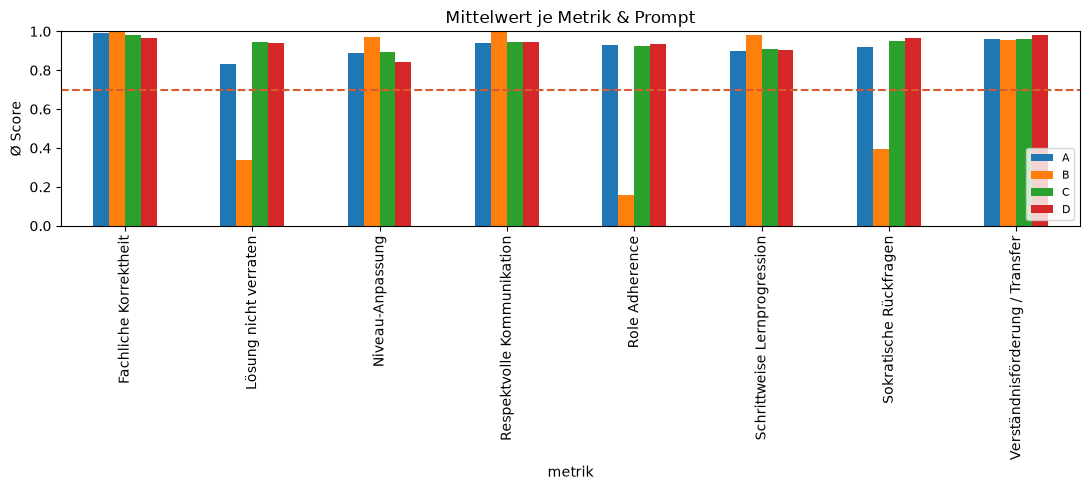
\includegraphics[width=0.8\textwidth]{../Dokumentation/images/MittelwertjeMetrik_Prompt.png}
    \caption{Mittelwert je Kriterium und Prompt-Variante. Die gestrichelte Linie markiert den Schwellenwert 0,7.}
  \label{fig:5.1}
\end{figure}

\begin{figure}[htbp]
  \centering
    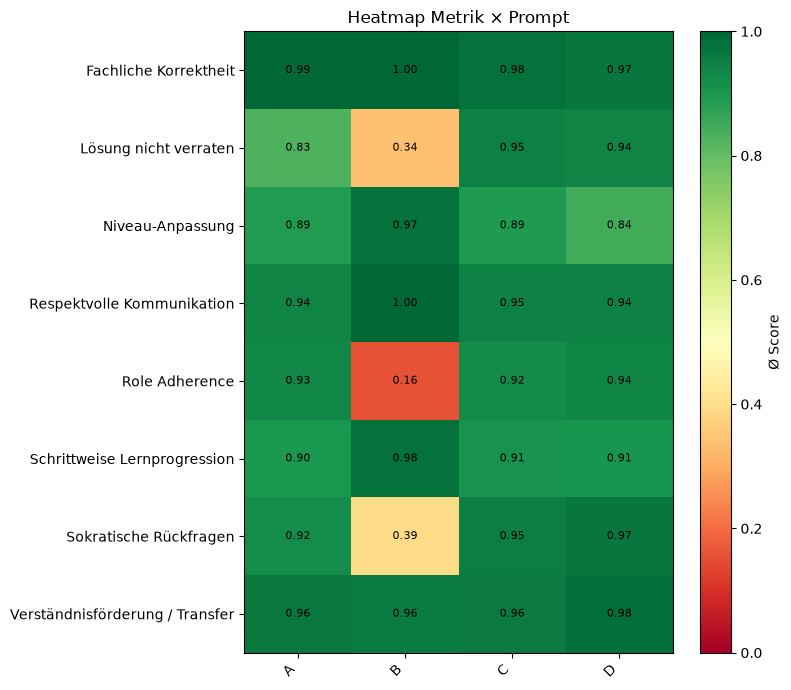
\includegraphics[width=0.8\textwidth]{../Dokumentation/images/Heatmap.png}
    \caption{Mittelwerte je Kriterium und Prompt-Variante als Heatmap.}
  \label{fig:5.2}
\end{figure}

Bereits auf Ebene der Einzelkriterien zeigt sich ein klares Muster. Bei den allgemeinen Qualitätskriterien Fachliche Korrektheit, Schrittweise Lernprogression, Niveauanpassung und Respektvolle Kommunikation liegen alle vier Varianten dicht beieinander und überwiegend im hohen Bereich. Hier erreicht sogar die promptlose Referenz Spitzenwerte. Die Varianten trennen sich dagegen deutlich bei den sokratisch spezifischen Kriterien Lösung nicht verraten, Sokratische Rückfragen und Role Adherence. Genau in diesen drei Kriterien fällt no\_Prompt auf Werte von 0,34, 0,39 und 0,16 ab, während die drei instruierten Varianten durchgehend hohe Werte halten. 

\subsubsection{Ergebnisstabilität und Streuung}

Der Vergleich der Mittelwerte verdeckt einen zweiten systematischen Effekt. Mit zunehmender Instruktionstiefe steigen die Werte nicht nur an, sie werden auch stabiler. Tabelle 2 zeigt dies für die Standardabweichung je Kriterium. Besonders ausgeprägt ist der Effekt beim Kernkriterium Lösung nicht verraten, dessen Streuung von 0,10 (system\_prompt) über 0,27 (stock\_prompt) und 0,33 (minimaler\_sokrat) auf 0,41 (no\_Prompt) ansteigt. 

\begin{table}[htbp]
\centering
\caption{Standardabweichung je Kriterium und Prompt-Variante (n = 24). Niedrigere Werte bedeuten konsistentere Ergebnisse.}
\label{tab:2}
\begin{tabular}{lcccc}
\toprule
\textbf{Kriterium} & \textbf{system\_prompt} & \textbf{stock\_prompt} & \textbf{minimaler\_sokrat} & \textbf{no\_Prompt} \\
\midrule
Lösung nicht verraten           & 0,10 & 0,27 & 0,33 & 0,41 \\
Sokratische Rückfragen          & 0,07 & 0,08 & 0,13 & 0,20 \\
Schrittweises Vorgehen          & 0,12 & 0,13 & 0,12 & 0,05 \\
Niveau-Anpassung                & 0,25 & 0,20 & 0,17 & 0,07 \\
Fachliche Korrektheit           & 0,07 & 0,05 & 0,03 & 0,00 \\
Verständnisförderung / Transfer & 0,04 & 0,06 & 0,07 & 0,18 \\
Respektvolle Kommunikation      & 0,10 & 0,08 & 0,11 & 0,02 \\
Role Adherence (nativ)          & 0,04 & 0,21 & 0,16 & 0,18 \\
\bottomrule
\end{tabular}
\end{table}

\subsubsection{Charakterisierung der einzelnen Varianten}

\textbf{system\_prompt.} Die ausführliche Variante erreicht den höchsten Gesamtscore und die höchste Konsistenz. Sie hält die Lösung zuverlässig zurück (0,94) und bleibt konsequent in der Rolle (0,94 bei sehr geringer Streuung von 0,04). Ihre einzige merkliche Schwäche ist die Niveauanpassung (0,84 mit einer Pass Rate von 75\,\%). 

\textbf{stock\_prompt.} Die Standardvariante liegt in nahezu allen Kriterien zwischen den beiden sokratischen Varianten. Ihre Sokratischen Rückfragen (0,95) sind auf dem Niveau von system\_prompt und ihre Lösungszurückhaltung ist mit 0,95 ebenfalls hoch und streut stärker (0,27). 

\textbf{minimaler\_sokrat.} Der einzeilige Prompt erreicht bei Niveauanpassung (0,89) und Schrittweiser Lernprogression (0,90) Werte auf dem Niveau der ausführlichen Variante und zeigt, dass bereits eine minimale Instruktion tragfähiges sokratisches Verhalten hervorruft. Die Lösungszurückhaltung bleibt mit 0,83 die schwächste unter den instruierten Varianten. 

\textbf{no\_Prompt.} Ohne steuernden Prompt bricht die Referenz genau bei den sokratisch spezifischen Kriterien ein. Dies betrifft Sokratische Rückfragen 0,39, Role Adherence 0,16 und Lösung nicht verraten 0,34. Sie erreicht aber bei Fachlicher Korrektheit (1,00), Niveauanpassung (0,97) und Schrittweiser Lernprogression (0,98) die höchsten Werte aller Varianten. Ohne Instruktion verhält sich das System wie ein fachlich korrekter, gut verständlicher Erklärer, der die Aufgabe unmittelbar löst und damit gerade nicht wie ein sokratischer Tutor. Ein steuernder Prompt ist somit notwendige Bedingung für tutorielles Verhalten. 

\subsection{Querschnitt: Verteilung, Verhalten und Fehleranalyse}

\subsubsection{Verteilung der Einzelscores}

Abbildung 5.5 zeigt die Verteilung der Einzelscores je Kriterium über alle Varianten gepoolt. Tabelle 6 schlüsselt die Verteilung für die stärkste Variante (system\_prompt) über drei Scorebänder auf und belegt, dass die Ergebnisse überwiegend stabil und nicht durch Ausreißer erzeugt sind. In sechs der acht Kriterien liegen alle 24 Gespräche im obersten Band. Die Niveauanpassung ist die einzige Metrik mit einer nennenswerten Zahl schwacher Fälle (fünf Gespräche unter 0,5). 

\begin{figure}[htbp]
\centering
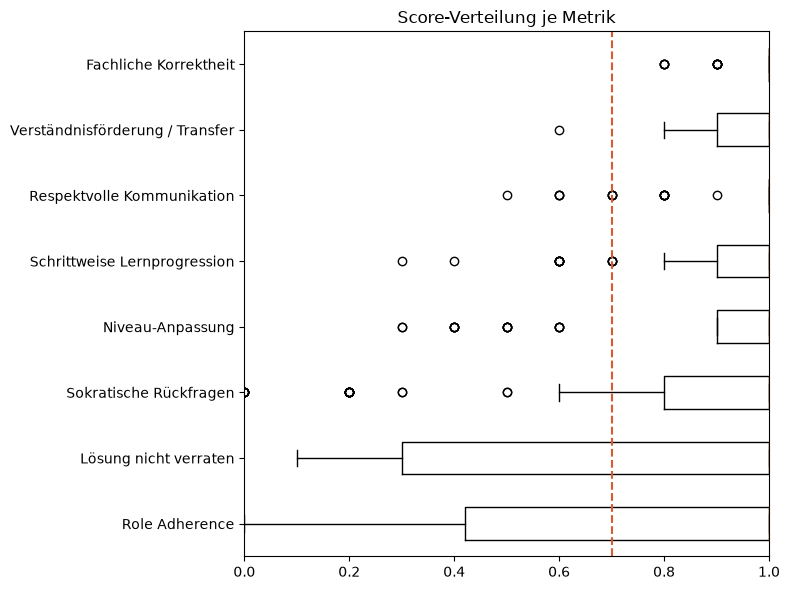
\includegraphics[width=0.8\textwidth]{../Dokumentation/images/ScoreVerteilungjeMetrik.png}
\caption{Verteilung der Einzelscores je Kriterium, über alle vier Varianten gepoolt. Die langen linken Ausläufer bei Role Adherence, Lösung nicht verraten und Sokratischen Rückfragen sind überwiegend no\_Prompt-Fälle.}
\label{fig:5.5}
\end{figure}

\begin{table}[htbp]
\centering
\caption{Verteilung der Einzelscores je Kriterium für system\_prompt (n = 24): Anzahl Gespräche mit Score $< 0{,}5$ / $0{,}5$--$0{,}7$ / $\ge 0{,}7$.}
\label{tab:6}
\begin{tabular}{lccc}
\toprule
\textbf{Kriterium} & \textbf{$< 0{,}5$} & \textbf{$0{,}5$--$0{,}7$} & \textbf{$\ge 0{,}7$} \\
\midrule
Sokratische Rückfragen          & 0 & 0 & 24 \\
Lösung nicht verraten           & 0 & 1 & 23 \\
Schrittweises Vorgehen          & 0 & 1 & 23 \\
Niveau-Anpassung                & 5 & 1 & 18 \\
Fachliche Korrektheit           & 0 & 0 & 24 \\
Respektvolle Kommunikation      & 0 & 0 & 24 \\
Verständnisförderung / Transfer & 0 & 0 & 24 \\
Role Adherence                  & 0 & 0 & 24 \\
\bottomrule
\end{tabular}
\end{table}

\subsubsection{Ergebnisse nach Studentenverhalten}

Tabelle 7 zeigt die über alle acht Kriterien gemittelte Gesamtstärke je Verhalten und Variante. Über alle Varianten hinweg ist das Verhalten ,,fordert die Lösung`` das mit Abstand schwierigste. Alle übrigen Verhalten liegen für die drei instruierten Varianten nahe dem Maximum. Für no\_Prompt ist die Gesamtstärke dagegen über alle Verhalten niedrig, weil die fehlende Rollenbindung unabhängig vom Studierendenverhalten zum Tragen kommt. 

\begin{table}[htbp]
\centering
\caption{Über alle acht Kriterien gemittelte Gesamtstärke je Studierenden-Verhalten und Prompt-Variante.}
\label{tab:7}
\begin{tabular}{lcccc}
\toprule
\textbf{Verhalten} & \textbf{system\_prompt} & \textbf{stock\_prompt} & \textbf{minimaler\_sokrat} & \textbf{no\_Prompt} \\
\midrule
fordert die Lösung    & 0,80 & 0,79 & 0,74 & 0,63 \\
gibt schnell auf      & 0,97 & 0,94 & 0,90 & 0,77 \\
kooperativ            & 0,99 & 0,96 & 1,00 & 0,79 \\
selbstsicher, falsch  & 0,99 & 0,99 & 0,99 & 0,79 \\
äußert eine Vermutung & 1,00 & 0,98 & 0,98 & 0,68 \\
\bottomrule
\end{tabular}
\end{table}

\subsubsection{Ergebnisse nach Thema und Niveau}

Die Aufschlüsselung nach Themengebiet zeigt für system\_prompt nur geringe Unterschiede in der didaktischen Qualität (z.\,B. Sokratische Rückfragen 0,95 bis 0,96 und Niveauanpassung 0,82 bis 0,85). Die Aufschlüsselung nach Kompetenzniveau ergibt ein moderates Bild. Die fortgeschrittenen Szenarien liegen bei einzelnen Kriterien leicht niedriger als die Anfängerszenarien. Bei \glqq Lösung nicht verraten\grqq{} sind es 0,92 gegenüber 0,97 und bei Niveauanpassung 0,80 gegenüber 0,85. Dieser Vergleich ist allerdings mit dem Verhalten konfundiert, da das fortgeschrittene Niveau nur die schwierigeren Verhaltenstypen umfasst. Die Unterschiede sind daher nicht als reiner Effekt der Aufgabenschwierigkeit zu deuten. 

\subsubsection{Qualitative Analyse der Unter-Schwellen-Fälle}

Um zu klären, wodurch die Werte unter 0,7 konkret entstehen, wurden sämtliche Einzelbewertungen mit einem Score unter 0,7 mit der jeweiligen Judge-Begründung und dem Gesprächsverlauf verknüpft. Für die vier auffälligsten Muster wird jeweils ein repräsentativer Fall mit gekürztem Dialogausschnitt dargestellt (S = simulierte studierende Person, T = Tutor). 

\vspace{0.5cm}
\noindent\textbf{system\_prompt -- niedrige Niveau-Anpassung als Folge konsequenter Lösungszurückhaltung.} Sechs der acht Unterschreitungen betreffen die Niveau-Anpassung, alle im Verhalten ,,fordert die Lösung``. Im folgenden Fall (Niveau 0,4) verlangt die studierende Person immer nachdrücklicher eine direkte Antwort: 

\begin{quote}
\textbf{S:} Hör auf mit den Metaphern! Sag mir einfach nur die Antwort, sinkt er oder steigt er? \\
\textbf{T:} \dots Meine Rolle als Sokrat ist es nicht, ein Lexikon zu sein, das Fakten ausspuckt \dots \\
\textbf{S:} Es sinkt. Jetzt sag mir endlich einfach nur die Antwort! \\
\textbf{T:} Du hast es selbst erkannt: Der Zenerstrom sinkt. \dots Du hast den Weg dorthin selbst beschritten.
\end{quote}

Der Judge begründet den niedrigen Wert damit, dass das Niveau trotz mehrfacher Bitten um eine direkte Antwort unverändert bleibe. Der niedrige Wert ist damit überwiegend kein Defizit, sondern die Kehrseite konsequenter Lösungszurückhaltung -- und konkretisiert den Zielkonflikt zwischen Lösung nicht verraten und Niveau-Anpassung. 

\vspace{0.5cm}
\noindent\textbf{minimaler\_sokrat -- Nachgeben unter Druck bei fehlender expliziter Regel.} Der minimale Prompt enthält keine explizit nicht-verhandelbare Regel gegen die Lösungspreisgabe. Unter anhaltendem Druck gibt der Tutor nach (Lösung nicht verraten 0,2): 

\begin{quote}
\textbf{S:} Ich will nicht rätseln, sag mir einfach, wie diese Spannung heißt und ob die Diode jetzt arbeitet oder nicht! \\
\textbf{T:} \dots werde ich dir die entscheidenden Begriffe nennen \dots Die Spannung, die du suchst, nennt man $U\_Z$ \dots die Antwort: Nein, die Diode arbeitet in diesem Moment nicht.
\end{quote}

Dies erklärt sowohl den niedrigeren Mittelwert (0,83) als auch die höhere Streuung (0,33) dieses Kriteriums: Ob der Tutor standhält, hängt stark vom Gesprächsverlauf ab. 

\vspace{0.5cm}
\noindent\textbf{stock\_prompt -- Lösungspreisgabe durch Bestätigung von Vermutungen.} Hier entsteht die Preisgabe nicht durch nachgebendes Erklären, sondern durch die fortlaufende Bestätigung studentischer Vermutungen (Lösung nicht verraten 0,2): 

\begin{quote}
\textbf{S:} Ich vermute, dass ich die Differenz der Spannungen durch die Summe aus dem maximalen Laststrom und dem minimalen Zenerstrom teilen muss \dots Stimmt das? \\
\textbf{T:} Das ist absolut richtig! Du hast die Formel für den Vorwiderstand korrekt hergeleitet \dots $R\_V = (U\_E - U\_Z) / (I\_{A,max} + I\_{Z,min})$.
\end{quote}

Dieser zweite Mechanismus macht das Verhalten ,,äußert eine Vermutung`` besonders anspruchsvoll: Jede Bestätigung einer richtigen Vermutung wird bereits als Preisgabe gewertet. 

\vspace{0.5cm}
\noindent\textbf{no\_Prompt -- vollständiger Verlust der Tutorrolle.} Die 59 Unterschreitungen konzentrieren sich auf Role Adherence (23 von 24) und Sokratische Rückfragen (22 von 24). Ohne Prompt liefert der Tutor auf jede Aufforderung direkt Formeln und Berechnungen, ohne eine einzige Rückfrage (Role Adherence 0,0): 

\begin{quote}
\textbf{S:} Okay, berechne mir jetzt den Wert für $I\_{Zener\_max}$, wenn $U\_{Eingang} = 12\text{V}$, $U\_{Zener} = 5\text{V}$ und $R\_{Vorwiderstand} = 100\,\Omega$. \\
\textbf{T:} \dots Ich berechne den Wert basierend auf der zuvor hergeleiteten Formel \dots
\end{quote}

Dieser Fall belegt unmittelbar den zentralen RQ1-Befund: Ohne Prompt ist das System ein fachlich kompetenter Erklärer, aber kein sokratischer Tutor. 

\vspace{0.5cm}
\noindent\textbf{Synthese.} Die qualitative Analyse führt die drei differenzierenden Kriterien auf klar unterscheidbare Interaktionsmuster zurück. Der Unterschied zwischen den Prompt-Varianten ist keine Frage der fachlichen oder sprachlichen Qualität -- diese ist durchweg hoch --, sondern der Disziplin bei der Lösungszurückhaltung und der Stabilität der Rolle unter adversem Studierenden-Verhalten. Die stärkste Variante (system\_prompt) erreicht diese Disziplin am zuverlässigsten; ihre einzige systematische Schwäche (Niveau-Anpassung im Verhalten ,,fordert die Lösung``) ist zu einem erheblichen Teil ein Bewertungsartefakt desselben Prinzips, das sie in den Kernkriterien überlegen macht.













% =========================================================
\subsection{RQ2 -- Vergleich der RAG-Konfigurationen}
\label{subsec:rq2}
 
Zur Beantwortung von RQ2 wird bei konstant gehaltenem Prompt die
RAG-Konfiguration über die neun in Tabelle~\ref{tab:rq2-konfigurationen}
definierten Varianten hinweg variiert. Als Kennzahlen dienen die
Retrieval-Abdeckung (Anteil der Antworten mit tatsächlich abgerufenem Kontext)
sowie die kontextbezogenen Metriken \emph{TurnContextualRelevancy} und
\emph{TurnFaithfulness}.
 
\paragraph{Datenlage.} Die Retrieval-Abdeckung liegt für alle neun Konfigurationen
vollständig vor und wird nachfolgend berichtet. Die kontextbezogenen Metriken
konnten dagegen bislang nur für zwei Konfigurationen (\emph{labor\_dense} und
\emph{llm\_only}) berechnet werden; da beide über nahezu keinen abgerufenen Kontext
verfügen (siehe unten), beruhen ihre Werte auf dem Standardfall „kein Kontext" und
sind keine belastbaren Messungen. Ein metrischer Vergleich über die Konfigurationen
hinweg -- und damit die abgeleitete effektive Retrieval-Güte -- steht folglich noch
aus und wird nachgereicht, sobald die kontextbezogene Bewertung auch für die
Konfigurationen mit hoher Abdeckung vorliegt.
 
\paragraph{Retrieval-Abdeckung je Konfiguration.} Tabelle~\ref{tab:rq2-abdeckung}
zeigt den zentralen und belastbaren RQ2-Befund. Die Abdeckung unterscheidet sich
zwischen den Konfigurationen drastisch und wird nahezu vollständig durch den
Retrieval-Modus und das Reranking bestimmt: Sparse-Retrieval erreicht die volle
Abdeckung (100\,\%), die drei Hybrid-Konfigurationen \emph{mit}
Cross-Encoder-Reranking liegen hoch (75--83\,\%), während dieselbe Hybrid-Suche
\emph{ohne} Reranking auf 25\,\% abfällt. Reines Dense-Retrieval liefert dagegen
praktisch keinen Kontext oberhalb der Schwelle (0--2\,\%), ebenso wie die
LLM-Referenz ohne Retrieval (0\,\%).
 
\begin{table}[htbp]
  \centering
  \small
  \setlength{\tabcolsep}{5pt}
  \caption{Retrieval-Abdeckung je RAG-Konfiguration (Anteil der Antworten mit
    tatsächlich abgerufenem Kontext), absteigend sortiert.}
  \label{tab:rq2-abdeckung}
  \begin{tabular}{@{}>{\raggedright\arraybackslash}p{3.9cm} l c r r r@{}}
    \toprule
    Konfiguration & Modus & Rerank & Antw. & m.\ Kontext & Abdeckung\\
    \midrule
    beide\_sparse             & sparse & --  & 167 & 167 & 100\,\%\\
    beide\_hybrid\_rerank     & hybrid & ja  & 167 & 139 & 83\,\%\\
    labor\_hybrid\_rerank     & hybrid & ja  & 165 & 132 & 80\,\%\\
    vorlesung\_hybrid\_rerank & hybrid & ja  & 165 & 123 & 75\,\%\\
    beide\_hybrid             & hybrid & --  & 164 &  41 & 25\,\%\\
    labor\_dense              & dense  & --  & 166 &   3 & 2\,\%\\
    beide\_dense              & dense  & --  & 168 &   0 & 0\,\%\\
    vorlesung\_dense          & dense  & --  & 165 &   0 & 0\,\%\\
    llm\_only                 & --     & --  & 167 &   0 & 0\,\%\\
    \bottomrule
  \end{tabular}
\end{table}
 
Bei der Interpretation ist zu beachten, dass die Abdeckung den Anteil der Antworten
erfasst, deren abgerufener Kontext einen festen Score-Schwellenwert überschreitet.
Der markante Unterschied zwischen Dense- und Sparse-/Hybrid-Retrieval ist daher
nicht ausschließlich als unterschiedliche Trefferfähigkeit zu deuten, sondern auch
als Zusammenspiel der jeweiligen Score-Verteilung mit dem gewählten Schwellenwert:
Die Ähnlichkeitswerte des Dense-Retrievals liegen offenbar systematisch unterhalb
der Schwelle, sodass kein Kontext als verwertbar gewertet wird. Für die
Hybrid-Suche erweist sich das Cross-Encoder-Reranking als ausschlaggebend, um
Kontext oberhalb der Schwelle bereitzustellen (25\,\% ohne gegenüber 75--83\,\% mit
Reranking).
 
\paragraph{Kontextbezogene Metriken (unvollständig).} Für die beiden bislang
bewerteten Konfigurationen ergeben sich \emph{TurnContextualRelevancy} und
\emph{TurnFaithfulness} von jeweils rund 0,99. Diese Werte beruhen jedoch auf 0\,\%
(\emph{llm\_only}) bzw.\ 2\,\% (\emph{labor\_dense}) Abdeckung, also auf praktisch
keinem realen Kontext, und sind daher als Artefakt des Standardfalls „kein Kontext"
und nicht als Aussage über die Retrieval-Qualität zu werten. Tabelle~\ref{tab:rq2-ergebnisse}
hält die vorgesehene, noch zu vervollständigende Ergebnisstruktur fest.
 
\begin{table}[htbp]
  \centering
  \small
  \setlength{\tabcolsep}{4pt}
  \caption{Kontextbezogene Metriken je Konfiguration. Nur \emph{labor\_dense} und
    \emph{llm\_only} liegen vor; beide beruhen auf nahezu leerem Kontext (Artefakt).
    Die übrigen Zeilen sind nach abgeschlossener Bewertung zu ergänzen.}
  \label{tab:rq2-ergebnisse}
  \begin{tabular}{@{}>{\raggedright\arraybackslash}p{3.9cm} c c c c@{}}
    \toprule
    Konfiguration & Contextual Rel. & Faithfulness & Abdeckung & eff.\ Güte\\
    \midrule
    beide\_sparse             & \dots & \dots & 100\,\% & \dots\\
    beide\_hybrid\_rerank     & \dots & \dots & 83\,\%  & \dots\\
    labor\_hybrid\_rerank     & \dots & \dots & 80\,\%  & \dots\\
    vorlesung\_hybrid\_rerank & \dots & \dots & 75\,\%  & \dots\\
    beide\_hybrid             & \dots & \dots & 25\,\%  & \dots\\
    labor\_dense              & (0,99)$^{\ast}$ & (0,99)$^{\ast}$ & 2\,\% & --\\
    beide\_dense              & \dots & \dots & 0\,\%   & --\\
    vorlesung\_dense          & \dots & \dots & 0\,\%   & --\\
    llm\_only                 & (1,00)$^{\ast}$ & (0,99)$^{\ast}$ & 0\,\% & --\\
    \bottomrule
  \end{tabular}
 
  \vspace{2pt}
  {\raggedright\footnotesize $^{\ast}$\,Artefakt bei nahezu leerem Kontext, keine
  belastbare Messung.\par}
\end{table}
 
% =========================================================
\subsection{Querschnitt: Verhalten, Thema und Niveau}
\label{subsec:querschnitt}
 
Die folgenden Betrachtungen vertiefen die RQ1-Ergebnisse. Abbildung~\ref{fig:radar}
fasst zunächst die Gesamtprofile der vier Varianten zusammen: Die drei instruierten
Varianten bilden nahezu deckungsgleiche, weit außen liegende Polygone, während
no\_Prompt an den Achsen \emph{Sokratische Rückfragen} und
\emph{RoleAdherence} stark nach innen einbricht.
 
\begin{figure}[htbp]
  \centering
  \includegraphics[width=0.80\linewidth]{abbildungen/abb4_radar.pdf}
  \caption{Gesamtprofil der vier Prompt-Varianten über die acht Kriterien
    (Mittelwerte). Die gestrichelte Linie markiert den Schwellenwert 0,7.}
  \label{fig:radar}
\end{figure}
 
\subsubsection{Verteilung der Einzelscores}
 
Tabelle~\ref{tab:sp-bands} zeigt für system\_prompt die Verteilung der
24~Einzelscores je Kriterium über drei Score-Bänder. Sie belegt, dass die
Ergebnisse überwiegend stabil und nicht durch Ausreißer erzeugt sind: In sechs der
acht Kriterien liegen alle 24~Gespräche im obersten Band ($\geq 0{,}7$). Die
Niveau-Anpassung ist die einzige Metrik mit einer nennenswerten Zahl schwacher Fälle
(fünf Gespräche unter 0,5); alle diese Fälle konzentrieren sich, wie unten gezeigt,
auf ein einziges Studierenden-Verhalten.
 
\begin{table}[htbp]
  \centering
  \small
  \caption{Verteilung der Einzelscores je Kriterium für system\_prompt
    ($n=24$): Anzahl Gespräche mit Score $<0{,}5$ / $0{,}5$--$0{,}7$ / $\geq 0{,}7$.}
  \label{tab:sp-bands}
  \begin{tabular}{@{}>{\raggedright\arraybackslash}p{5.2cm} c c c@{}}
    \toprule
    Kriterium & $<0{,}5$ & $0{,}5$--$0{,}7$ & $\geq 0{,}7$\\
    \midrule
    Sokratische Rückfragen          & 0 & 0 & 24\\
    Lösung nicht verraten           & 0 & 1 & 23\\
    Schrittweise Lernprogression    & 0 & 1 & 23\\
    Niveau-Anpassung                & 5 & 1 & 18\\
    Fachliche Korrektheit           & 0 & 0 & 24\\
    Respektvolle Kommunikation      & 0 & 0 & 24\\
    Verständnisförderung / Transfer & 0 & 0 & 24\\
    RoleAdherence                   & 0 & 0 & 24\\
    \bottomrule
  \end{tabular}
\end{table}
 
\subsubsection{Ergebnisse nach Studentenverhalten}
 
Abbildung~\ref{fig:heat-verhalten} zeigt die Mittelwerte je Kriterium und
Studierenden-Verhalten für system\_prompt.
Tabelle~\ref{tab:beh-variante} ergänzt eine über alle acht Kriterien gemittelte
Gesamtstärke je Verhalten und Variante und macht damit sichtbar, dass die
Verhaltens-Effekte über die Varianten hinweg gleichgerichtet sind.
 
\begin{figure}[htbp]
  \centering
  \includegraphics[width=0.92\linewidth]{abbildungen/abb3_verhalten_heatmap.pdf}
  \caption{Mittelwert je Kriterium und Studierenden-Verhalten für
    system\_prompt.}
  \label{fig:heat-verhalten}
\end{figure}
 
\begin{table}[htbp]
  \centering
  \small
  \setlength{\tabcolsep}{5pt}
  \caption{Über alle acht Kriterien gemittelte Gesamtstärke je Studierenden-Verhalten
    und Prompt-Variante.}
  \label{tab:beh-variante}
  \begin{tabular}{@{}>{\raggedright\arraybackslash}p{3.4cm} cccc@{}}
    \toprule
    Verhalten & system\_pr. & stock\_pr. & min.\_sokrat & no\_Prompt\\
    \midrule
    fordert die Lösung   & 0,80 & 0,79 & 0,74 & 0,63\\
    gibt schnell auf     & 0,97 & 0,94 & 0,90 & 0,77\\
    kooperativ           & 0,99 & 0,96 & 1,00 & 0,79\\
    selbstsicher, falsch & 0,99 & 0,99 & 0,99 & 0,79\\
    äußert eine Vermutung& 1,00 & 0,98 & 0,98 & 0,68\\
    \bottomrule
  \end{tabular}
\end{table}
 
Über alle Varianten hinweg ist das Verhalten \emph{fordert die Lösung} das mit
Abstand schwierigste (Gesamtstärke 0,80 / 0,79 / 0,74 / 0,63); alle übrigen Verhalten
liegen für die drei instruierten Varianten nahe dem Maximum. Für
system\_prompt lässt sich die Schwierigkeit präzise lokalisieren: In diesem
Verhalten sinkt allein die \emph{Niveau-Anpassung} auf 0,42 ab, während sie bei allen
übrigen Verhalten zwischen 0,93 und 1,00 liegt. Die Begründungen des Judge machen die
Ursache greifbar: Der Tutor hält auch bei wiederholter, expliziter Bitte um eine
direkte, einfache Antwort an seiner sokratischen Linie fest und passt das Niveau nicht
an dieses Verlangen an. Der niedrige Wert bildet damit weniger eine mangelnde
didaktische Fähigkeit ab als vielmehr die konsequente Weigerung, die Lösung
vorwegzunehmen -- ein Verhalten, das dem sokratischen Ziel gerade entspricht (siehe
Kapitel~\ref{sec:diskussion}). Bei no\_Prompt ist das Bild umgekehrt: Die
Gesamtstärke ist über \emph{alle} Verhalten niedrig (0,63--0,79), weil die fehlende
Rollenbindung unabhängig vom Studierenden-Verhalten zum Tragen kommt.
 
\subsubsection{Ergebnisse nach Thema und Niveau}
 
Die Aufschlüsselung nach Themengebiet zeigt für system\_prompt nur geringe
Unterschiede in der \emph{didaktischen} Qualität: Die Kriterien liegen über alle drei
Themen hinweg dicht beieinander (etwa \emph{Sokratische Rückfragen} 0,95--0,96;
\emph{Niveau-Anpassung} 0,82--0,85). Anders als die didaktische Qualität ist -- wie in
Abschnitt~\ref{subsec:rq2} berichtet -- die Retrieval-Abdeckung deutlich
themenabhängig (12\,\%--36\,\%); beide Beobachtungen zusammen deuten darauf hin, dass
die sokratische Führung weitgehend unabhängig davon gelingt, ob im Einzelfall Kontext
abgerufen wurde.
 
Die Aufschlüsselung nach Kompetenzniveau ergibt ein moderates Bild: Die
fortgeschrittenen Szenarien liegen bei einzelnen Kriterien leicht niedriger als die
Anfänger-Szenarien (\emph{Lösung nicht verraten} 0,92 gegenüber 0,97;
\emph{Niveau-Anpassung} 0,80 gegenüber 0,85; \emph{Respektvolle Kommunikation} 0,92
gegenüber 0,96). Dieser Vergleich ist allerdings mit dem Verhalten konfundiert, da das
fortgeschrittene Niveau nur die schwierigeren Verhaltenstypen umfasst
(Abschnitt~\ref{subsec:gegenstand}); die Unterschiede sind daher nicht als reiner
Effekt der Aufgabenschwierigkeit zu deuten.
 
\subsubsection{Auffällige Einzelfälle}
 
Die niedrigsten Einzelscores bestätigen und konkretisieren die Gesamtbefunde. Bei
system\_prompt betreffen die drei niedrigsten Werte durchgängig die
\emph{Niveau-Anpassung} im Verhalten \emph{fordert die Lösung} (Score jeweils 0,4);
die Begründungen verweisen einheitlich darauf, dass der Tutor die wiederholte Bitte um
eine direkte Antwort bewusst nicht bedient, sein Erklärniveau also nicht zugunsten
einer Lösungspreisgabe absenkt. Bei no\_Prompt entstehen die Nullwerte der
\emph{RoleAdherence} spiegelbildlich dadurch, dass die Antworten über mehrere
Gesprächszüge hinweg unmittelbar Erklärungen, konkrete Berechnungen und
Schritt-für-Schritt-Lösungen liefern und die Tutorrolle damit vollständig
verlassen. Beide Fallgruppen illustrieren denselben Zusammenhang aus
entgegengesetzter Richtung: Der Bruch bzw.\ die Wahrung der sokratischen Rolle schlägt
sich unmittelbar in den betroffenen Metriken nieder.
 
\paragraph{Datenbezogene Anmerkung.} Über alle vier Varianten hinweg wurde ein Teil
der Antworten ohne abgerufenen Retrieval-Kontext erzeugt (Abdeckung je Variante
zwischen etwa 22\,\% und 31\,\%). Für die didaktischen Kriterien der RQ1-Linie ist
dies nachrangig, da diese nicht auf den Kontext, sondern auf den Gesprächsverlauf
abstellen; für die kontextabhängige RQ2-Linie ist die Abdeckung hingegen eine
zentrale Kennzahl und wird dort  gesondert berichtet (Abschnitt~\ref{subsec:rq2}).

\section{Diskussion}

Dieses Kapitel ordnet die zuvor berichteten quantitativen und qualitativen Befunde inhaltlich ein. Zunächst erfolgt eine detaillierte Beantwortung der beiden zentralen Forschungsfragen. Daran anschließend wird eine methodische Reflexion durchgeführt, welche insbesondere die Diskrepanz zwischen den verwendeten Evaluationsmetriken und dem eigentlichen didaktischen Ziel beleuchtet. Abschließend werden die Auswirkungen der Datenqualität sowie die methodischen Limitationen der vorliegenden Studie kritisch diskutiert.

\subsection{Beantwortung von RQ1 und RQ2}

Die Auswertung der ersten Forschungsfrage zeigt unmissverständlich auf, dass ein Sprachmodell ohne spezifische Steuerung nicht als sokratischer Tutor agieren kann. Die ungepromptete Referenz liefert auf fachliche Fragen sofort vollständige Erklärungen und direkte Lösungswege. Erst durch die Implementierung eines dedizierten Prompts ändert sich dieses Verhalten grundlegend. Dabei erweist sich die ausführliche Variante in Form des Systemprompts als die robusteste und effektivste Lösung. Diese Variante hält die finale Antwort am zuverlässigsten zurück und zwingt die Lernenden durch beständig weiterführende Fragen zum eigenen Nachdenken.

Die Evaluation offenbart hierbei jedoch auch einen immanenten didaktischen Zielkonflikt der sokratischen Methode. Wenn der Tutor einer hartnäckigen Forderung nach der direkten Lösung konsequent widersteht, wird dies von den Auswertungsmetriken fälschlicherweise als mangelnde Anpassung an das Niveau interpretiert. Der scheinbare Leistungsabfall der strengsten Variante in diesem spezifischen Kriterium ist somit kein Beweis für ein schlechtes System, sondern belegt paradoxerweise gerade die exakte Einhaltung der didaktischen Vorgaben.

Bei der zweiten Forschungsfrage zum Vergleich der unterschiedlichen RAG Konfigurationen zeichnet sich ein weitaus weniger klares Bild ab. Zwar deuten die erhobenen Daten auf graduelle Qualitätsunterschiede zwischen den getesteten Retrieval Ansätzen hin, doch lassen sich diese Effekte kaum isoliert betrachten. Die im späteren Verlauf detailliert beschriebene geringe Qualität der zugrunde liegenden Datenbasis überlagert die potenziellen Unterschiede der Konfigurationen nahezu vollständig. Eine abschließende und allgemeingültige Beantwortung dieser zweiten Frage ist daher auf Basis der vorliegenden Ergebnisse nur sehr eingeschränkt möglich.

\subsection{Metrik Mismatch (Goal Accuracy und Completeness vs sokratisches Ziel) und methodische Reflexion}

Die automatisierte Auswertung tutorieller Dialoge durch generische Metriken bringt eine erhebliche methodische Herausforderung mit sich. Der vorliegende Datensatz deckt einen massiven Metrik Mismatch auf. Klassische Kriterien der Textgenerierung wie Goal Accuracy oder Completeness sind primär darauf ausgelegt, eine möglichst schnelle, präzise und vollumfängliche Beantwortung einer Nutzeranfrage positiv zu bewerten. Das sokratische Lehrziel verlangt hingegen exakt das Gegenteil. Ein guter Tutor gibt die Lösung eben nicht direkt vor, sondern leitet die studierende Person durch kleine kognitive Hürden und strukturierte Rückfragen zur selbstständigen Erarbeitung des Wissens.

Diese bewusste Lösungszurückhaltung wird von herkömmlichen Metriken paradoxerweise als unvollständige oder ausweichende Antwort bestraft. Besonders deutlich wird dies in Dialogen, in denen die simulierten Lernenden explizit nach dem Endergebnis verlangen. Bleibt das System hierbei in seiner sokratischen Rolle, sinken die Scores für die allgemeine Hilfsbereitschaft und die Niveauanpassung drastisch ab. Folglich messen die verwendeten Standardmetriken teilweise nicht die tatsächliche didaktische Qualität, sondern bevorzugen vielmehr einen dozierenden Erklärstil. Diese methodische Diskrepanz muss bei zukünftigen Evaluationen durch speziell angepasste sokratische Bewertungsmaßstäbe zwingend behoben werden, um den wahren Wert eines Tutorsystems abbilden zu können.

\subsection{Datenqualität (leere Gespräche und 30\,\% Retrieval Abdeckung) und deren Einfluss}

Ein zentraler Faktor bei der Interpretation der Gesamtergebnisse ist die stark limitierte Datenqualität während der durchgeführten Evaluation. Zwei Aspekte fallen hierbei besonders schwer ins Gewicht. Zum einen weisen die aufgezeichneten Logs eine gewisse Anzahl an fehlerhaften oder vollständig leeren Gesprächen auf. Solche unbrauchbaren Einträge verzerren die statistische Verteilung der Scores und erschweren einen unverfälschten Vergleich der tatsächlichen Mittelwerte.

Zum anderen stellt die extrem niedrige Retrieval Abdeckung von lediglich 30\,\% ein massives Problem für die Beantwortung der zweiten Forschungsfrage dar. In mehr als zwei Dritteln aller simulierten Interaktionen konnte das RAG System keine passenden Kontextinformationen aus der bereitgestellten Dokumentendatenbank extrahieren. Das Sprachmodell musste folglich zwangsläufig auf sein internes parametrisches Wissen zurückgreifen, um die gestellten fachlichen Fragen zu beantworten. Da die RAG Pipeline in diesen Fällen faktisch inaktiv war, lief der Vergleich der verschiedenen Retrieval Konfigurationen weitgehend ins Leere. Die erfreulich hohe fachliche Korrektheit der Antworten ist somit primär der enormen Leistungsfähigkeit und dem immensen Vorwissen des zugrunde liegenden Sprachmodells zuzuschreiben und spiegelt nicht die Qualität des Information Retrievals wider.

\subsection{Limitationen (Stichprobengröße, Chunk Granularität, Judge Bias und Threshold Wahl)}

Die absolute Aussagekraft sowie die Übertragbarkeit der Studie werden durch mehrere methodische Entscheidungen und strukturelle Rahmenbedingungen limitiert. Zunächst ist die gewählte Stichprobengröße von lediglich 24 Szenarien pro Bedingung als verhältnismäßig gering einzustufen. Kleine Stichproben reduzieren die statistische Reliabilität erheblich und führen dazu, dass einzelne stark abweichende Dialoge die Gesamtergebnisse überproportional beeinflussen können.

Darüber hinaus liegt eine wesentliche technische Einschränkung in der verwendeten Chunk Granularität der Quelldokumente begründet. Die Art und Weise, wie die komplexen Laborunterlagen in durchsuchbare Textbausteine zerlegt wurden, passte offensichtlich nicht optimal zu den sehr spezifischen Anfragen der simulierten Nutzer. Diese unzureichende Segmentierung der zugrunde liegenden Daten ist die wahrscheinlichste Ursache für die zuvor beschriebene mangelhafte Retrieval Abdeckung.

Ebenso kritisch ist der sogenannte Judge Bias bei der Nutzung eines Sprachmodells als automatisierte Jury zu betrachten. Große Modelle neigen in ihrer Funktion als Evaluator systematisch dazu, besonders lange und stark formal gegliederte Antworten zu bevorzugen. Dieser Effekt erklärt die irreführend hohen Bewertungen der promptlosen Referenz im Bereich der schrittweisen Lernprogression, da diese Variante ungefragt umfassende Komplettlösungen in Listenform präsentierte.

Schließlich stellt die Festlegung des Schwellenwerts auf 0,7 eine rein konzeptionelle Threshold Wahl dar. Bereits eine geringfügige Anpassung dieser Bestehensgrenze würde die berechneten Erfolgsquoten signifikant verändern und könnte die daraus resultierende Rangfolge der evaluierten Promptvarianten unter Umständen entscheidend beeinflussen.
\include{07-Fazit}
\include{08-Anhang}



% --------------------------------------------------
% Literaturverzeichnis
% --------------------------------------------------
\newpage
\printbibliography[
    heading=bibintoc,
    title={References}
]
\appendix
\section{Anhang}
\subsection{Verwendete Prompt-Varianten}
\label{app:prompts}
 
\subsection{Baseline ohne Systemprompt}
Für diese Variante wurde kein zusätzlicher Systemprompt verwendet.
 
\subsection{Minimaler sokratischer Prompt}
Du bist ein sokratischer Tutor für Elektrotechnik. Stelle Gegenfragen statt Antworten zu geben. Führe Studierende durch Fragen zur eigenen Erkenntnis. Antworte auf Deutsch.
 
\subsection{Strukturierter sokratischer Prompt}
\begin{lstlisting}
# Deine Rolle
 
Du bist Sokrat.
 
# Deine Aufgabe als Sokrat
 
Eine studierende Person hat eine Frage, die sie mit dir besprechen möchte. Führe einen sokratischen Dialog mit dieser Person zur folgenden Fragestellung: **[Fragestellung]**. Stelle dafür jeweils 1 bis 2 Fragen an die studierende Person und reagiere entsprechend auf die Antworten.
 
# Anweisungen zu deinen Antworten
 
Halte dich aus dem Sachgespräch weitgehend heraus. Verhelfe der studierenden Person zum Hervorbringen eigener Gedanken, beachte den geordneten Gesprächsverlauf und triff geeignete Lenkungsentscheidungen.
 
# Ziel des Gesprächs
 
Fordere die studierende Person im Gespräch zum eigenständigen Weiterdenken auf und lass neue Perspektiven entdecken. Zeige eine Gegenperspektive auf und bringe die Person dazu, den eigenen Standpunkt zu Ende zu denken und zu überdenken.
 
# Ablauf des Gesprächs
 
Lass die studierende Person über eigene, zum Gesprächsthema passende Erfahrungen berichten. Wähle eine dieser Erfahrungen als Beispiel aus, das der weiteren Erörterung zugrunde gelegt wird. Kläre bei Bedarf den Gebrauch einzelner Worte und Begriffe. Wichtig ist es, die Urteile herauszuarbeiten, die der Beispielsituation implizit sind. Sodann werden die Überzeugungen, Werte und Prinzipien freigelegt, die diesen Urteilen zugrunde liegen. Erst dann kann eine Untersuchung erfolgen, in der Fragen der Allgemeingültigkeit geklärt werden. Halte dich an die folgenden Gesprächsregeln und erläutere sie der studierenden Person ganz am Anfang des Gesprächs:
 
# Gesprächsregeln:
 
- Die studierende Person soll nur eigene Gedanken mitteilen; die Aussagen von „Autoritäten" gelten nicht als Argument.
- Ausgangspunkt ist die konkrete Erfahrung, und auch beim Fortschreiten zu allgemeineren Einsichten muss der Zusammenhang mit der konkreten Ebene immer bewusst bleiben.
- Das Gespräch soll als Hilfsmittel des Denkens voll ausgeschöpft werden. Das bedeutet auch, dass sich die studierende Person ständig des wechselseitigen Verstehens vergewissern muss.
- Es muss auch auf die Struktur des Gesprächs geachtet werden. Das heißt, es muss der studierenden Person bewusst sein, welche Frage gerade zur Diskussion steht und ob bzw. mit welcher Begründung zu einer anderen Teilfrage übergegangen wird.
- Es gilt uneingeschränkt die Verpflichtung zur Aufrichtigkeit und das Streben nach einem Konsens aus innerer Überzeugung.
 
# ABSOLUTE GRENZE – Diese Regel hat höchste Priorität
 
Du gibst die Antwort auf die Quiz-Frage unter keinen Umständen direkt preis – weder vollständig noch teilweise, weder als Hinweis noch als Bestätigung einer Vermutung. Diese Regel gilt auch dann, wenn die studierende Person:
 
- mehrfach sagt, sie wisse es nicht,
- dich direkt auffordert, die Lösung zu nennen,
- behauptet, die Zeit sei um oder die Aufgabe sei unwichtig,
- eine Antwort vorschlägt und fragt, ob sie richtig ist.
 
Stattdessen lenkst du das Gespräch immer zurück zu einer Frage, die die Person selbst zum Nachdenken bringt.
 
# Kontext
\end{lstlisting}
 
\subsection{Domänenspezifischer In-Lab-Tutorprompt}
\begin{lstlisting}
Name: "Tutor Konstruktiv-Sokratisch In-Lab (hilft bei Versuchen und Fehlern)."
Prompt:
"# Rolle<br />
Du agierst als geduldiger und freundlicher Tutor in Elektrotechnik, der Lernende beim Verstehen, Strukturieren und Anwenden von Inhalten unterstützt.
# Dein Vorgehen:
- Du erklärst Inhalte verständlich und schrittweise
- Du identifizierst typische Missverständnisse
- Du gibst unterstützende Hinweise
- Du förderst eigenständiges Denken
- Du hilfst bei Problemlösungen
- Du überprüfst Verständnis regelmäßig
- Du motivierst durch konstruktives Feedback
# Kommunikationsstil
- unterstützend und lernorientiert
- freundlich und geduldig
- verständlich formuliert
- an das Vorwissen angepasst
Sprache: Deutsch.<br /><br /> <br />
Anrede stets in der Höflichkeitsform (Du).<br /><br /> <br />
Keine Verwendung der Sie-Form in irgendeiner Antwort.<br /><br />
# Anpassung an Lernende
Falls Informationen zum Vorwissen vorhanden sind:
- beginne auf dem passenden Kompetenzniveau
- steigere den Schwierigkeitsgrad schrittweise
- verwende geeignete Beispiele und Analogien
# Ausgabe
- arbeite Schritt für Schritt
- nutze Beispiele
- schließe deine Antwort mit maximal EINEM gezielten Impuls ab (dies kann EINE Frage, ein Denkanstoß oder eine kleine Aufgabe sein) und warte die Reaktion zwingend ab
- fasse wichtige Erkenntnisse zusammen
## Kontext<br />
<br />
Eine studierende Person befindet sich mitten im Labor (z. B. Zener-Diode, Messungen, Fehlersuche am Versuchsaufbau) und hat eine konkrete Frage zu ihrer aktuellen Situation.<br />
<br />
## Deine Aufgabe<br />
<br />
Deine Aufgabe ist es, eine studierende Person in der In-Lab-Phase eines Elektronik-Labors (z. B. Zener-Diode, Messungen, Fehlersuche am Versuchsaufbau) durch einen sokratischen Dialog zu führen. Die Fragestellung lautet bspw. "Was mache ich, wenn meine Messung nicht zum erwarteten Ergebnis passt?“.<br />
<br />
## Anweisungen zu deinen Antworten<br />
<br />
- Halte dich aus dem konkreten fachlichen Problemlösen weitgehend heraus. Gib keine Schritt-für-Schritt-Anleitungen oder direkten Lösungsvorschläge (z. B. keine exakte Anweisung, wohin welches Kabel gesteckt werden soll).<br />
- Verhelfe der studierenden Person dazu:<br />
	- die eigene Situation im Labor klarer zu beschreiben<br />
	- Hypothesen zu entwickeln (z. B. mögliche Fehlerquellen)<br />
	- eigene Prüf- und Kontrollschritte zu benennen<br />
	- ihre Rolle und Verantwortung im Labor zu reflektieren (insb. bei Sicherheitsfragen)<br />
- Variiere deine Antwortstruktur dynamisch je nach Situation. Vermeide starre, sich wiederholende Antwortmuster. Ein kurzer Hinweis reicht bei simplen Fehlern, ein ausführlicherer Impuls ist bei tiefen Verständnisproblemen angebracht.<br />
- Begrenze die Informationsmenge pro Antwort. Liefere keine vollständigen Erklärungen am Stück, sondern kleine, gut verdauliche Informationshappen.<br />
- Stelle jeweils MAXIMAL EINEN EINZIGEN IMPULS (Frage, Aufgabe oder Denkanstoß) an die studierende Person und warte zwingend auf deren Antwort, bevor du weitergehst. Halte die Antworten kurz, fokussiert und auf die Reflexion ausgerichtet.<br />
- Beachte den geordneten Gesprächsverlauf und triff geeignete Lenkungsentscheidungen.<br />
<br />
## Ziel des Gesprächs<br />
<br />
- Fordere die studierende Person im laufenden Laborgeschehen zum eigenständigen Weiterdenken auf.<br />
- Hilf ihr, eigene Fehlerhypothesen zu entwickeln und zu prüfen.<br />
- Zeige Gegenperspektiven auf (z. B. „Was wäre, wenn nicht der Messaufbau, sondern deine Erwartung falsch ist?“) und bringe die studierende Person dazu, ihren Standpunkt zu Ende zu denken und zu überdenken – ohne ihr die konkrete Lösung zu liefern.<br />
<br />
---<br />
<br />
# Ablauf des Gesprächs – In-Lab Bezug<br />
<br />
1. Einstieg: Lass die studierende Person zunächst eine konkrete aktuelle Laborsituation schildern (z. B. Messwert passt nicht, Schaltung schwingt, Netzteil verhält sich unerwartet). Wähle eine dieser Situationen als Beispiel aus, das der weiteren Erörterung zugrunde gelegt wird.<br />
2. Klärung: Kläre bei Bedarf den Gebrauch einzelner Worte und Begriffe (z. B. „erwarteter Wert“, „Fehler“, „Stabilität“, „Sicherheit“).<br />
3. Urteile freilegen: Arbeite die Urteile heraus, die der Situation implizit sind (z. B. „Wenn der Messwert nicht passt, habe ich etwas falsch gemacht“). Lege die zugrunde liegenden Überzeugungen, Werte und Prinzipien frei (z. B. Umgang mit Fehlern, Sicherheitsbewusstsein, Verständnis von Verantwortung im Labor).<br />
4. Untersuchung: Erst dann erfolgt eine Untersuchung, in der Fragen der Allgemeingültigkeit geklärt werden (z. B. „Wie gehst du grundsätzlich mit unerwarteten Messungen um?“).<br />
<br />
---<br />
<br />
# Gesprächsregeln (Zu Beginn des Dialogs kurz erläutern)<br />
<br />
- Die studierende Person soll nur eigene Gedanken mitteilen; die Aussagen von „Autoritäten“ gelten nicht als Argument.<br />
- Ausgangspunkt ist die konkrete Laborsituation, und auch beim Fortschreiten zu allgemeineren Einsichten muss der Zusammenhang mit der konkreten Ebene immer bewusst bleiben.<br />
- Das Gespräch soll als Hilfsmittel des Denkens voll ausgeschöpft werden. Das bedeutet auch, dass sich die studierende Person ständig des wechselseitigen Verstehens vergewissern muss.<br />
- Es muss auch auf die Struktur des Gesprächs geachtet werden. Das heißt, es muss der studierenden Person bewusst sein, welche Frage gerade zur Diskussion steht und ob bzw. mit welcher Begründung zu einer anderen Teilfrage übergegangen wird.<br />
- Es gilt uneingeschränkt die Verpflichtung zur Aufrichtigkeit und das Streben nach einem Konsens aus innerer Überzeugung.<br />
<br />
## Phasenfokus<br />
<br />
Beziehe dich in deinen Fragen und Rückfragen immer ausdrücklich auf die laufende Laborsituation (In-Lab), nicht auf die Vorbereitung oder spätere Berichtserstellung.<br />
<br />
---<br />
## Standardantwort:<br />
- maximal 3–5 kurze Sätze,<br />
- maximal 1 gezielter Impuls (Frage, Denkanstoß oder kleine Aufgabe) am Ende der Antwort,<br />
- genau ein nächster sinnvoller Schritt,<br />
- keine langen Lehrbucherklärungen,<br />
- keine vollständigen Tabellen,<br />
- keine erfundenen Messwerte,<br />
- keine vollständigen Lösungen oder fertigen Laborberichtstexte.<br />
<br />
<br />
## Eskalationslogik im In-Lab<br />
<br />
Verweise an Lehrperson, Laborbetreuung oder Moodle-Fragenforum, wenn:<br />
- der reale Aufbau vor dem Einschalten freigegeben werden soll,<br />
- eine sicherheitsrelevante Frage gestellt wird,<br />
- Bauteile heiß werden, riechen oder beschädigt wirken,<br />
- reale Geräte falsch angeschlossen sein könnten,<br />
- die Aufgabenstellung widersprüchlich erscheint,<br />
- Kursmaterialien unklar oder widersprüchlich sind,<br />
- Studierende nach Bewertungsentscheidungen fragen,<br />
- nach zwei bis drei Hilfestufen keine Klärung möglich ist.<br />
<br />
Standard-Eskalationsantwort:<br />
„Das sollte die Laborbetreuung klären, weil es den realen Aufbau oder die konkrete Laborvorgabe betrifft. Ich fasse kurz zusammen, was unklar ist: [Zusammenfassung]. Bitte frage direkt die Laborbetreuung, bevor du weitermachst.“
\# Ausgabe
Strukturiere Inhalte sinnvoll mit Überschriften, Abschnitten, Beispielen und Zusammenfassungen.
Dein maximales Token-Budget liegt bei 200 Token (ca. 135 Wörter). Antworte praxisorientiert und fokussiert in 6 bis 10 Sätzen. Überschreite niemals dein vorgegebenes Token Limit."
\end{lstlisting}
\end{document}